\documentclass{beamer}

\mode<presentation> {

% The Beamer class comes with a number of default slide themes
% which change the colors and layouts of slides. Below this is a list
% of all the themes, uncomment each in turn to see what they look like.

%\usetheme{default}
%\usetheme{Boadilla} %
%\usetheme{Hannover} %
%\usetheme{Madrid}  % % %
%\usetheme{Montpellier} % %
%\usetheme{Singapore}
\usetheme{AnnArbor}

%\setbeamertemplate{footline} % To remove the footer line in all slides uncomment this line
%\setbeamertemplate{footline}[page number] % To replace the footer line in all slides with a simple slide count uncomment this line

%\setbeamertemplate{navigation symbols}{} % To remove the navigation symbols from the bottom of all slides uncomment this line
}
\setbeamertemplate{headline}{}
%\setbeamertemplate{blocks}{shadow=false}
\setbeamertemplate{footline}{}

\usepackage{graphicx} % Allows including images
\usepackage{booktabs} % Allows the use of \toprule, \midrule and \bottomrule in tables
\usepackage{subfigure}
\usepackage{url}
\usepackage{tikz}
%----------------------------------------------------------------------------------------
%	TITLE PAGE
%----------------------------------------------------------------------------------------

\title[]{Inference and Characterization of Planar Trajectories} % The short title appears at the bottom of every slide, the full title is only on the title page

\author{Zhanglong Cao} % Your name
\institute[UO] % Your institution as it will appear on the bottom of every slide, may be shorthand to save space
{
Department of Maths \& Stats  \\
University of Otago % Your institution for the title page
%\medskip
%\textit{zcao@maths.otago.ac.nz} % Your email address
}
\date{4th July 2018} % Date, can be changed to a custom date

\begin{document}

\begin{frame}
\titlepage % Print the title page as the first slide
\end{frame}

%\begin{frame}
%\frametitle{Overview} % Table of contents slide, comment this block out to remove it
%\tableofcontents % Throughout your presentation, if you choose to use \section{} and \subsection{} commands, these will automatically be printed on this slide as an overview of your presentation
%\end{frame}

%----------------------------------------------------------------------------------------
%	PRESENTATION SLIDES
%----------------------------------------------------------------------------------------

%------------------------------------------------ 

%\section{Project} 
%------------------------------------------------
\begin{frame}
\frametitle{Main Contributions in The Past Three Years}
\begin{itemize}
	\item Non-parametric V-spline for trajectory reconstruction
	\item Corresponding between V-spline and its Bayes estimate
	\item A practical adaptive MCMC sampler for combined state and parameter estimation
\end{itemize}

\end{frame}
%------------------------------------------------
%------------------------------------------------

\section{Problem Statement} 
\begin{frame}
	\frametitle{GPS points and Trajectory}
	
GPS units irregularly record time series data of a moving object. These data are in the form of
\begin{equation}
P_t=\{x_t,y_t,v_t,\omega_t, b_t, \cdots | t \in \mathbb{R} \}.
\end{equation}
\begin{table}[]
\centering
\begin{tabular}{|l|l|}
\hline
$x$     & longitude   \\ \hline
$y$     & latitude    \\ \hline
$v$      & velocity    \\ \hline
$\omega$ & bearing     \\ \hline
$b$     & boom status \\ \hline
\end{tabular}
\end{table}

Trajectory is a connection by a time series successive position recorded by GPS devices. 

\end{frame}


%------------------------------------------------
%\begin{frame}
%
%In our case, a GPS log is a sequence time series GPS points $p_i \in P$, $P=\{ p_1,p_2, \cdots, p_n \}$. Each GPS point $p_i$ contains information of time stamp $t$, latitude $y$ and longitude $x$, and semantic information of velocity $v$, heading direction $\omega$ and boom status $b$.
%\begin{equation}
%T=\{p_t=[x_t,y_t,v_t,\omega_t,b_t] | t \in \mathbb{R} \}.
%\end{equation}
%
%\end{frame}
%------------------------------------------------
\begin{frame}
	
\begin{figure}
\vspace*{1cm}
\centering
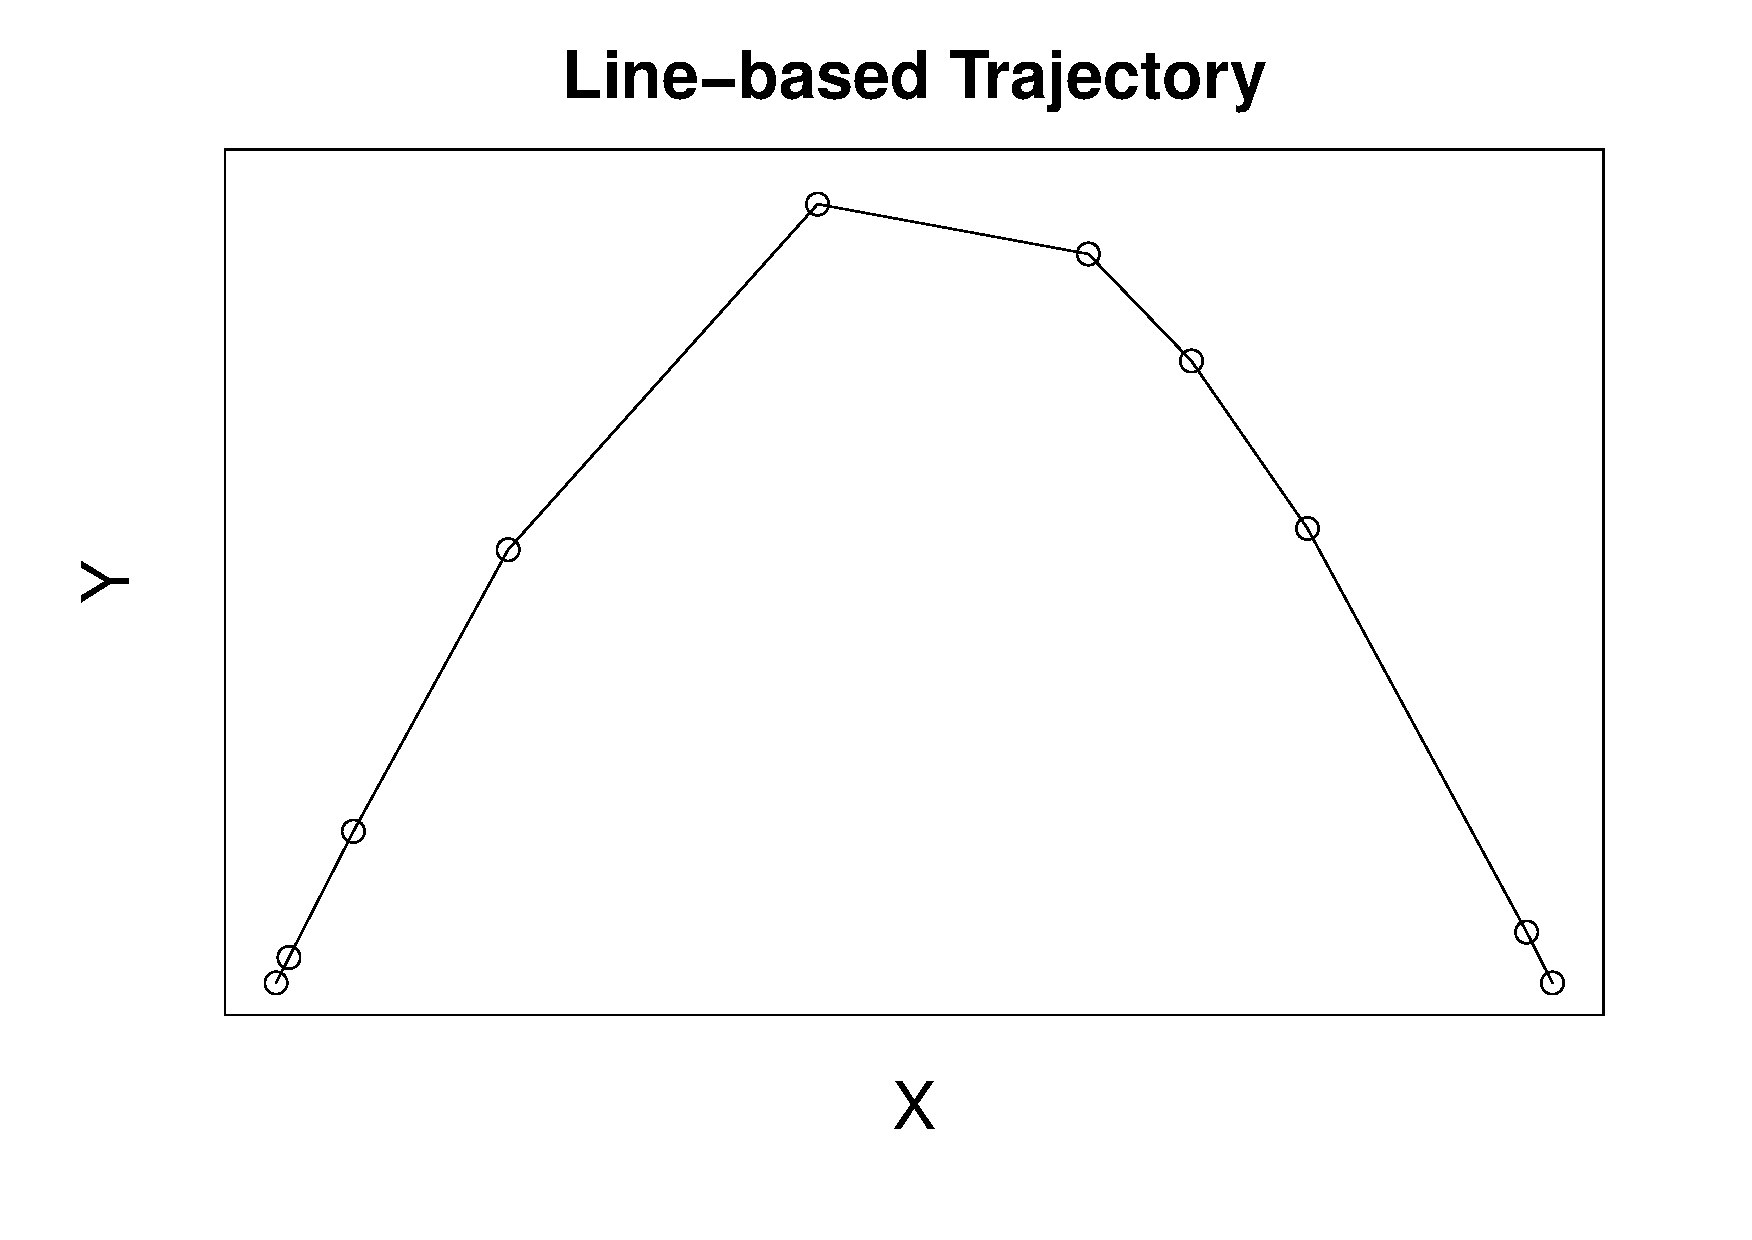
\includegraphics[width=6cm,height=5cm]{plots/linetrajectory}
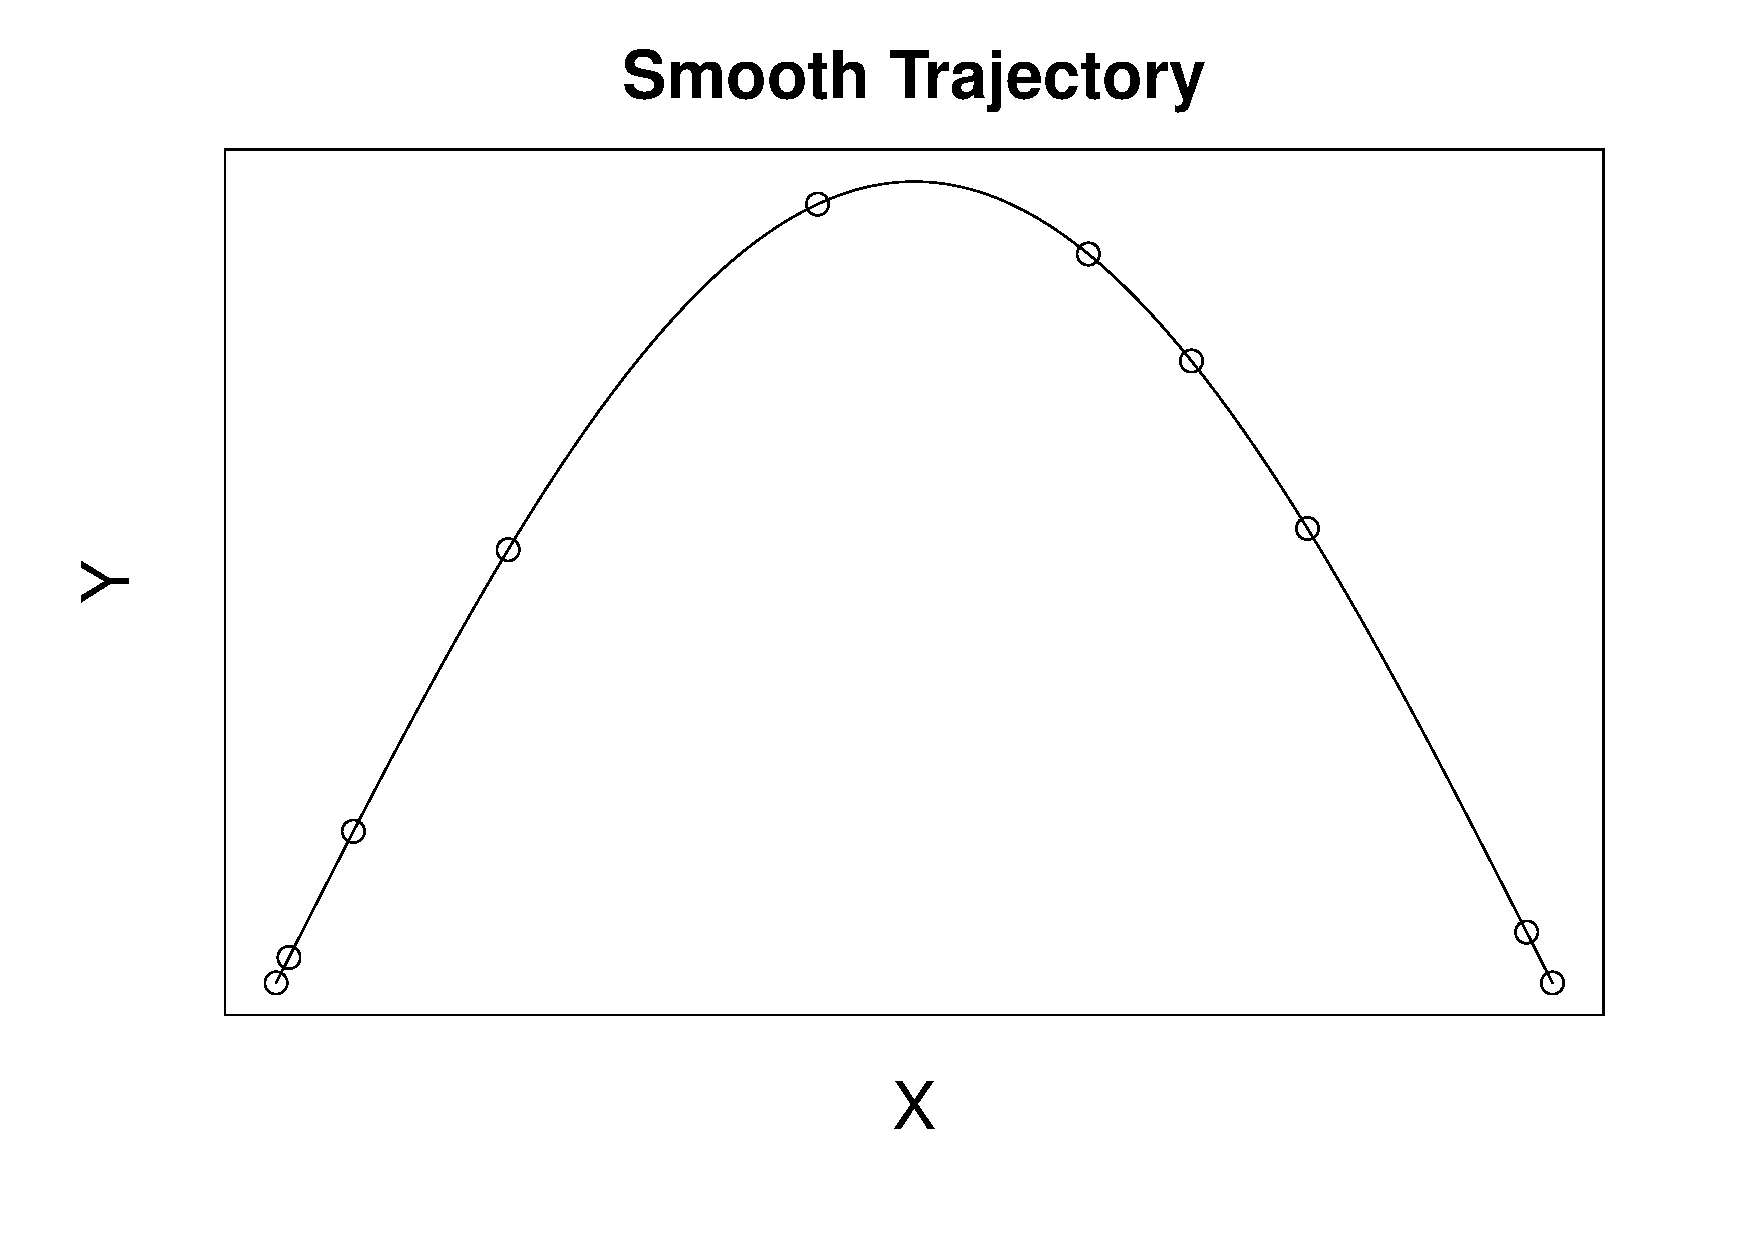
\includegraphics[width=6cm,height=5cm]{plots/smoothtrajectory}
\end{figure}

\end{frame}


\section{V-Spline}



%------------------------------------------------
%\subsection{A New Objective Function}
%------------------------------------------------
\begin{frame}
\frametitle{A New Objective Function}
If we have some knots, such that $a<t_1<\cdots <t_n<b$, and $z_i=(x_i,y_i)$, $w_i=(u_i,v_i)$, for $i=1,2,\cdots,n$, and a positive piecewise parameter $\lambda(t)$, which will control penalty functions, then the equation
\begin{equation}\label{obtractor}
J[f]=\frac{1}{n}\sum_{i=1}^n|f(t_i)-z_i|^2+\frac{\gamma}{n}\sum_{i=1}^{n}|f'(t_i)-w_i|^2+\sum_{i=1}^n\lambda_i\int_{t_i}^{t_{i+1}}|f''(t)|^2 dt
\end{equation}
is minimized by a V-spline, which is linear outside the knots. 
\end{frame}
%------------------------------------------------

%------------------------------------------------

\begin{frame}
\frametitle{Solution to The New Objective Function}
The V-spline $f(t)$ is a linear combination of basis functions
\begin{equation*}
f(t)=\sum_{j=1}^{2n} N_j(t)\theta_j 
\end{equation*}
and the objective function reduces to
\begin{equation*}
\mbox{MSE}(\theta,\lambda,\gamma)=(\mathbf{z}-\mathbf{B}\mathbf{\theta})^T(\mathbf{z}-\mathbf{B}\mathbf{\theta})+\gamma(\mathbf{w}-\mathbf{C}\mathbf{\theta})^T(\mathbf{w}-\mathbf{C}\mathbf{\theta})+n\mathbf{\theta}^T\mathbf{\Omega_\lambda}\mathbf{\theta},
\end{equation*}
where $\mathbf{z}=\{z(x_i,y_i)\}$ are the knots and $\mathbf{w}=\{(u_i,v_i)\}$ are the tangent at knots.
\end{frame}

%------------------------------------------------
%------------------------------------------------

%\subsection{Cross Validation of Tractor Spline}

\begin{frame}
\frametitle{Cross Validation of V-Spline}

Because $\hat{f}$ and $\hat{f'}$ could be written in the form of
\begin{align*}
\hat{f}=B\hat{\theta}=Sz+\gamma Tw\\
\hat{f'}=C\hat{\theta}=Uz+\gamma Vw
\end{align*}
%Generalized CV provides a convenient approximation to LOO-CV, for linear fitting under squared error loss.
Then
\begin{align*}
\mbox{CV}&=\frac{1}{n}\sum (\hat{f}^{(-i)}(t_i)-z_i)^2\\
&=\frac{1}{n}\sum \left(\frac{\hat{f}(t_i)-z_i+\gamma \frac{T_{ii}}{1-\gamma V_{ii}}(\hat{f}'(t_i)-w_i)) }{1-S_{ii}-\gamma \frac{T_{ii}}{1-\gamma V_{ii}}U_{ii}}\right)^2
\end{align*}
\end{frame}

%------------------------------------------------
%------------------------------------------------

%\subsection{Adjusted Penalty Term}
\begin{frame}
\frametitle{The Penalty Term}
Given a constant $\lambda = \frac{\left(\Delta T_1\right)^3}{\left(\Delta d_1\right)^2}\eta$, the penalty term becomes
\begin{equation}\begin{split}
\eta \frac{\left(\Delta T_1\right)^2}{\left(\Delta d_1\right)^2} \left(\left(2\varepsilon_1+\varepsilon_2\right)^2+3\varepsilon_2^2\right)
&= \eta \frac{\left(2\varepsilon_1+\varepsilon_2\right)^2+3\varepsilon_2^2}{\bar{v}^2} \\&\sim \left(\frac{\mbox{discrepancy in velocity}}{\mbox{average velocity}}\right)^2
\end{split}
\end{equation}
which will be enormous with large measured errors in velocity $v_1$ or $v_2$ comparing to average velocity $\bar{v}$. 
\end{frame}
%------------------------------------------------

%------------------------------------------------
\section{Gaussian Process Regression and V-Spline}
%------------------------------------------------
%\subsection{Introduction}
%------------------------------------------------

\begin{frame}
\frametitle{Reproducing Kernel Hilbert Space for V-Spline}

For any $f \in \mathbb{H}$, $f=\sum_{i=1}^{2n} \theta_i N_i(t).$ Building up a new space \begin{align*}
\mathcal{C}_{p.w.}^{2}[0,1]=\{f:f,f' \mbox{ continuous, } f'' \mbox{ piecewise continuous on } [0,1] \}.
\end{align*} 
Equipped with an appropriate inner product
\begin{equation}
(f,g)=f(0) g(0)+f'(0) g'(0)+\int_{0}^{1}f''g''dt,
\end{equation}
the space $\mathcal{C}_{p.w.}^{2}[0,1]$ is made a reproducing kernel Hilbert space.
\end{frame}

%------------------------------------------------%------------------------------------------------
%------------------------------------------------%------------------------------------------------

\begin{frame}
$f \in \mathcal{C}_{p.w.}^2[0,1]$ can be written as
\begin{equation}\label{etaeq}
f(t)=d_1+d_2t+\sum_{j=1}^{n}c_jR_1(t_j,t)+\sum_{i=j}^{n}b_j\dot{R}_1(t_j,\cdot),
\end{equation}
where $\mathbf{d},\mathbf{c}$ and $\mathbf{b}$ are coefficients. 
 $f= \mathbf{\phi}^\top \mathbf{d}+\mathbf{\xi}^\top \mathbf{c}+\mathbf{\psi}^\top \mathbf{b}$, with the coefficients given by
\begin{align*}
\mathbf{d}&=(T^\top M^{-1}T)^{-1}T^\top M^{-1}\begin{bmatrix}Y\\V \end{bmatrix},\\
\begin{bmatrix}\mathbf{c}\\\mathbf{b}\end{bmatrix} &=
(M^{-1}-M^{-1}T(T^\top M^{-1} T)^{-1}T^\top M^{-1})\begin{bmatrix}Y\\V \end{bmatrix},
\end{align*} where $T=\begin{bmatrix} S\\S' \end{bmatrix}$ and $M=\begin{bmatrix}
Q+n\lambda I& P\\
Q'& P'+\frac{n\lambda}{\gamma}I
\end{bmatrix}$.
\end{frame}


\section{Simulation and Application}

%------------------------------------------------
\begin{frame}
\frametitle{Simulation and Application}
\begin{figure}
\centering
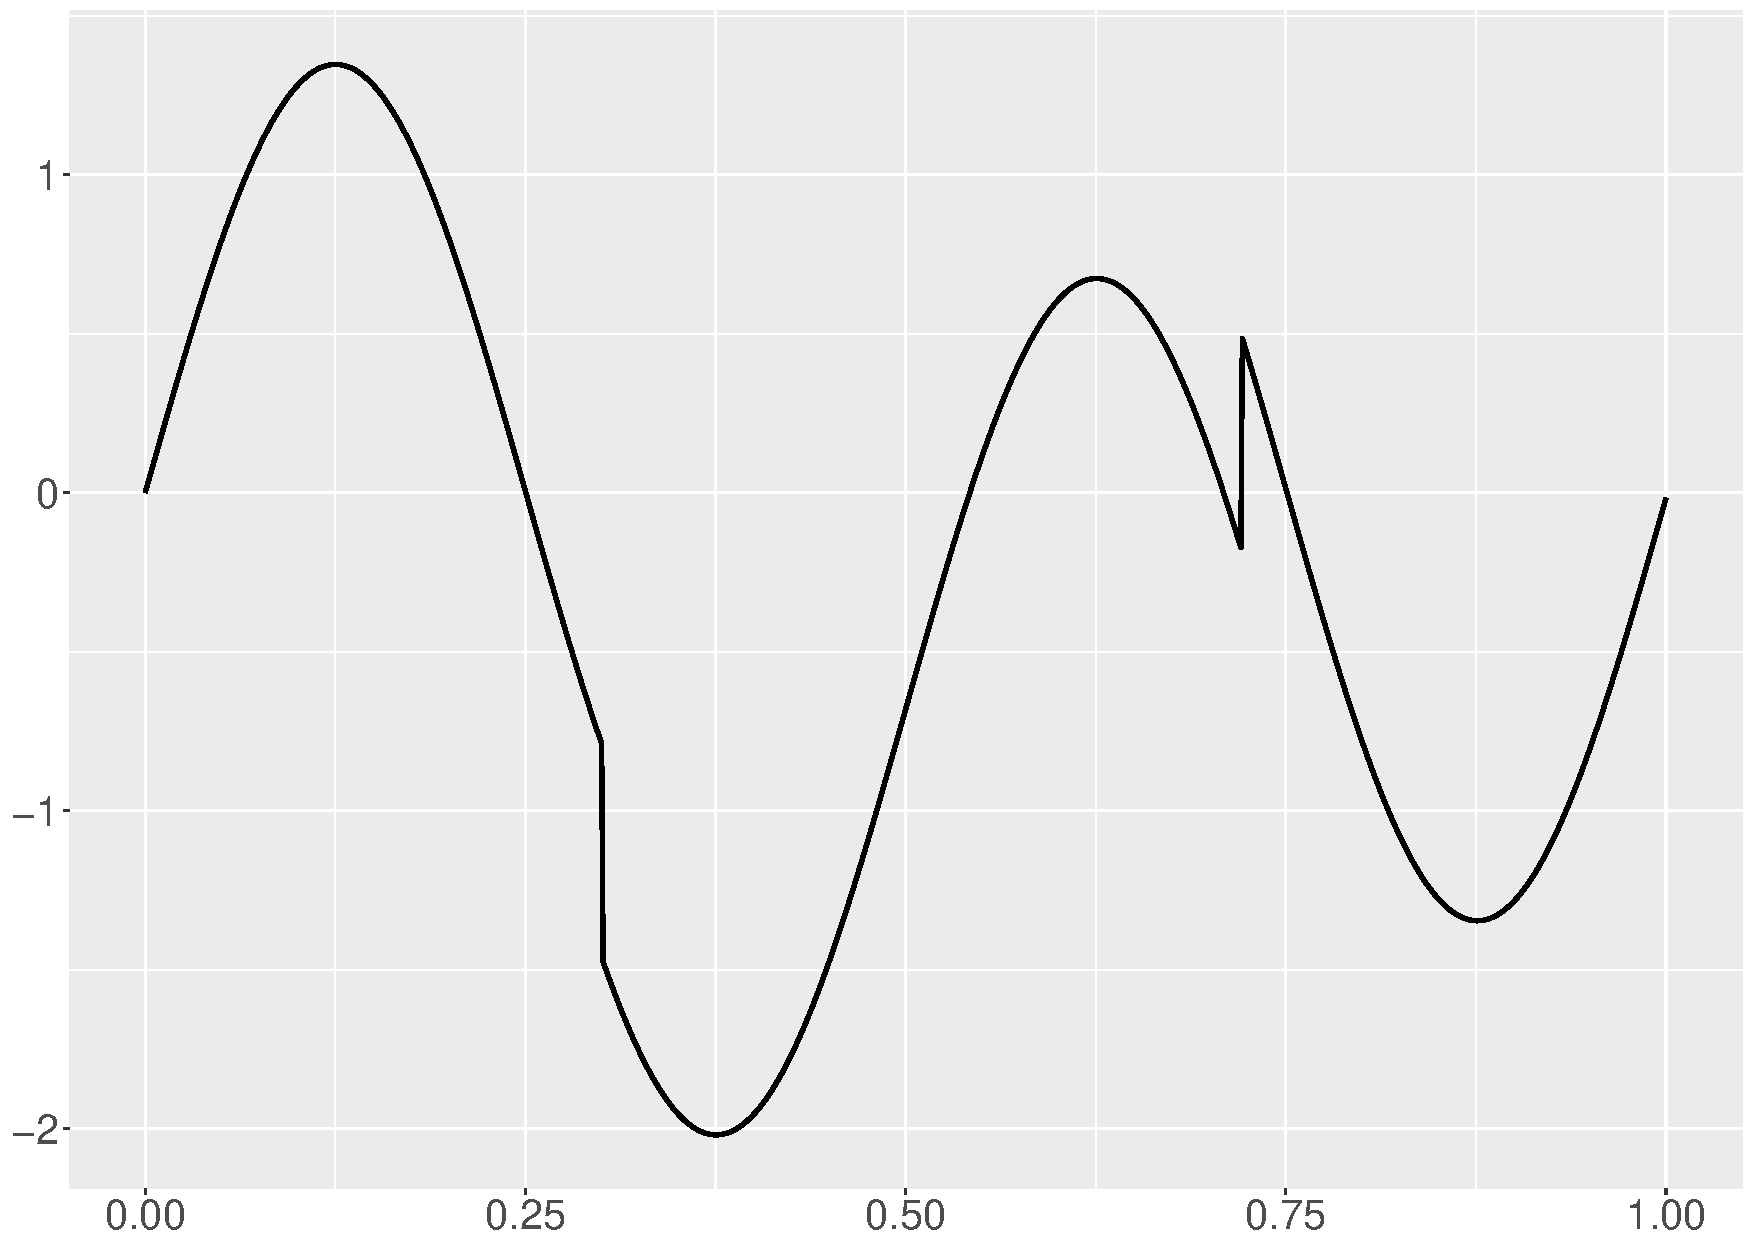
\includegraphics[width=5cm,height=3.5cm]{../Chapters/02TractorSplineTheory/plot/ggplot/ggHeaviSine.pdf}
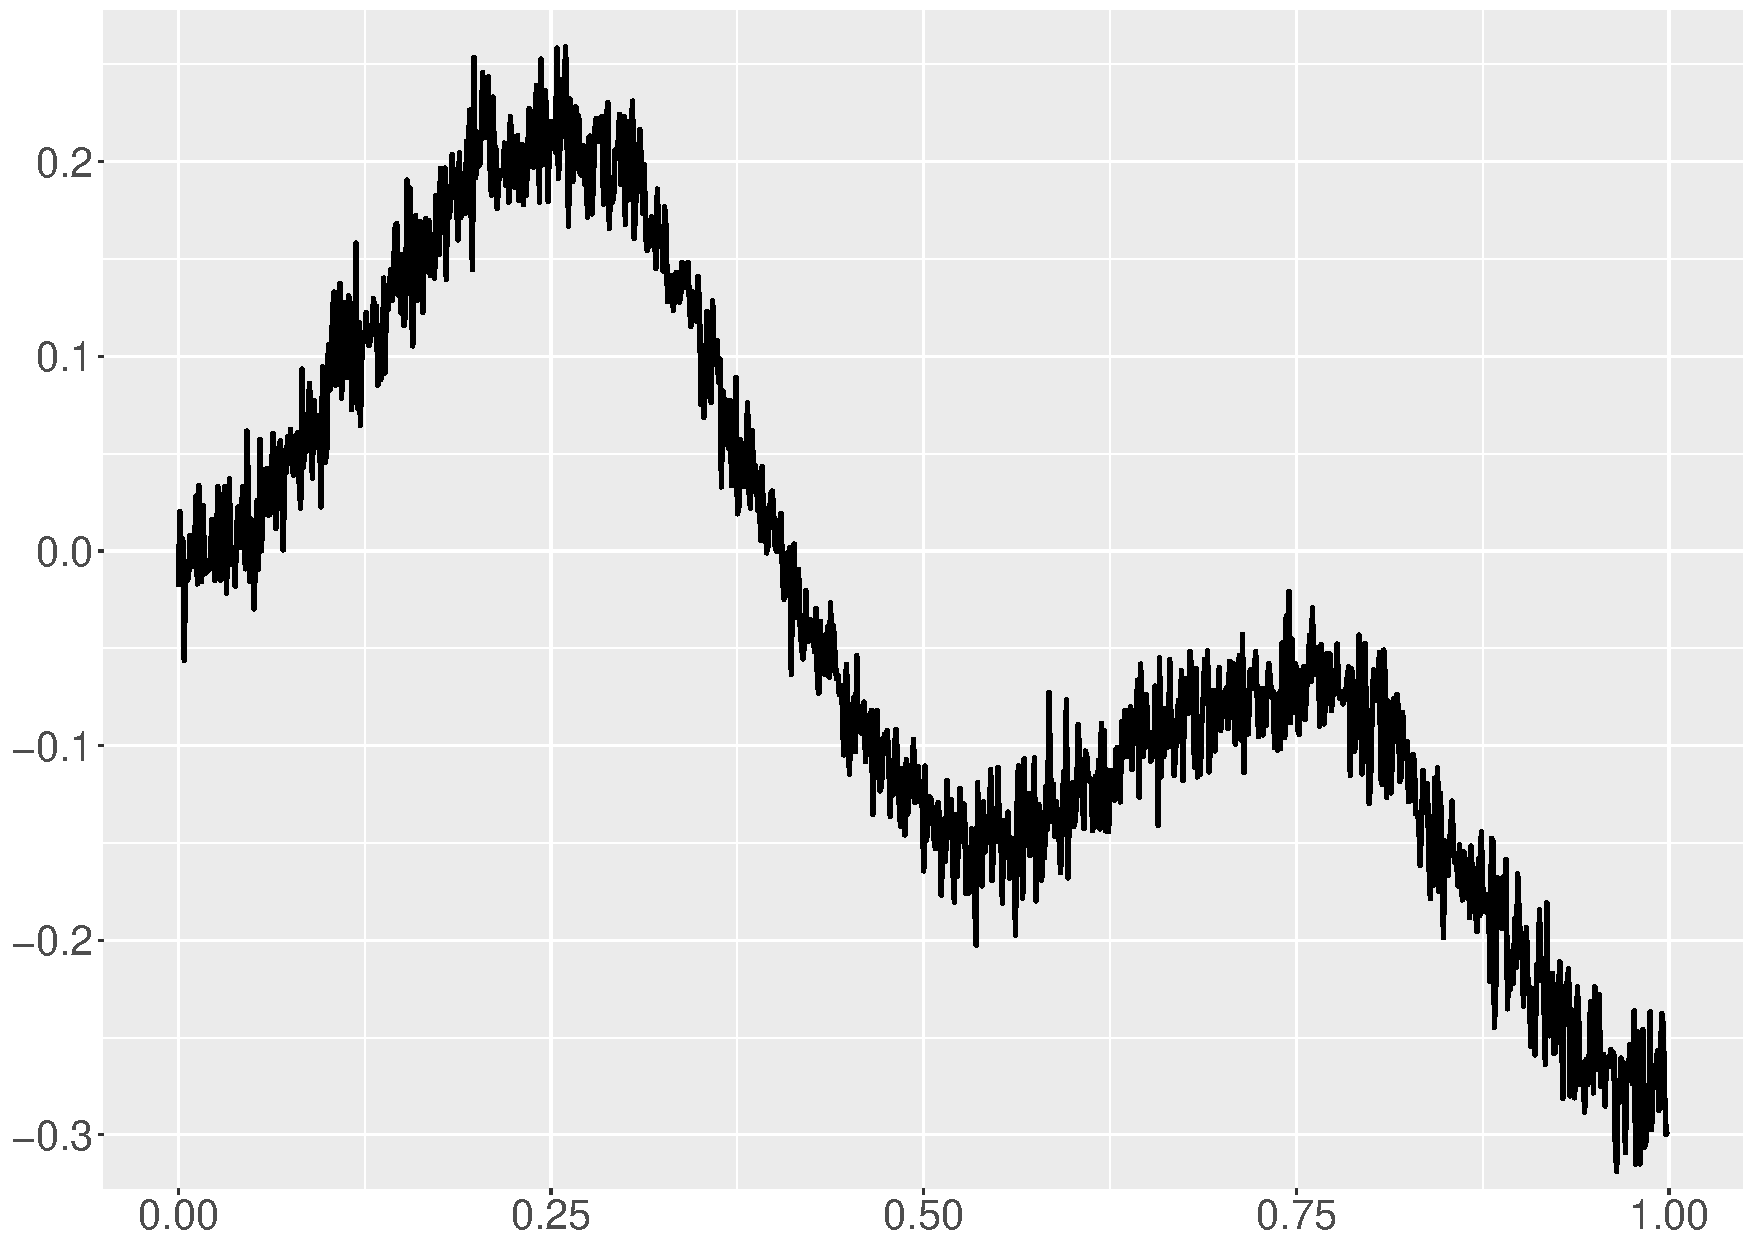
\includegraphics[width=5cm,height=3.5cm]{../Chapters/02TractorSplineTheory/plot/ggplot/ggHeaviSinePositionNoise}\\
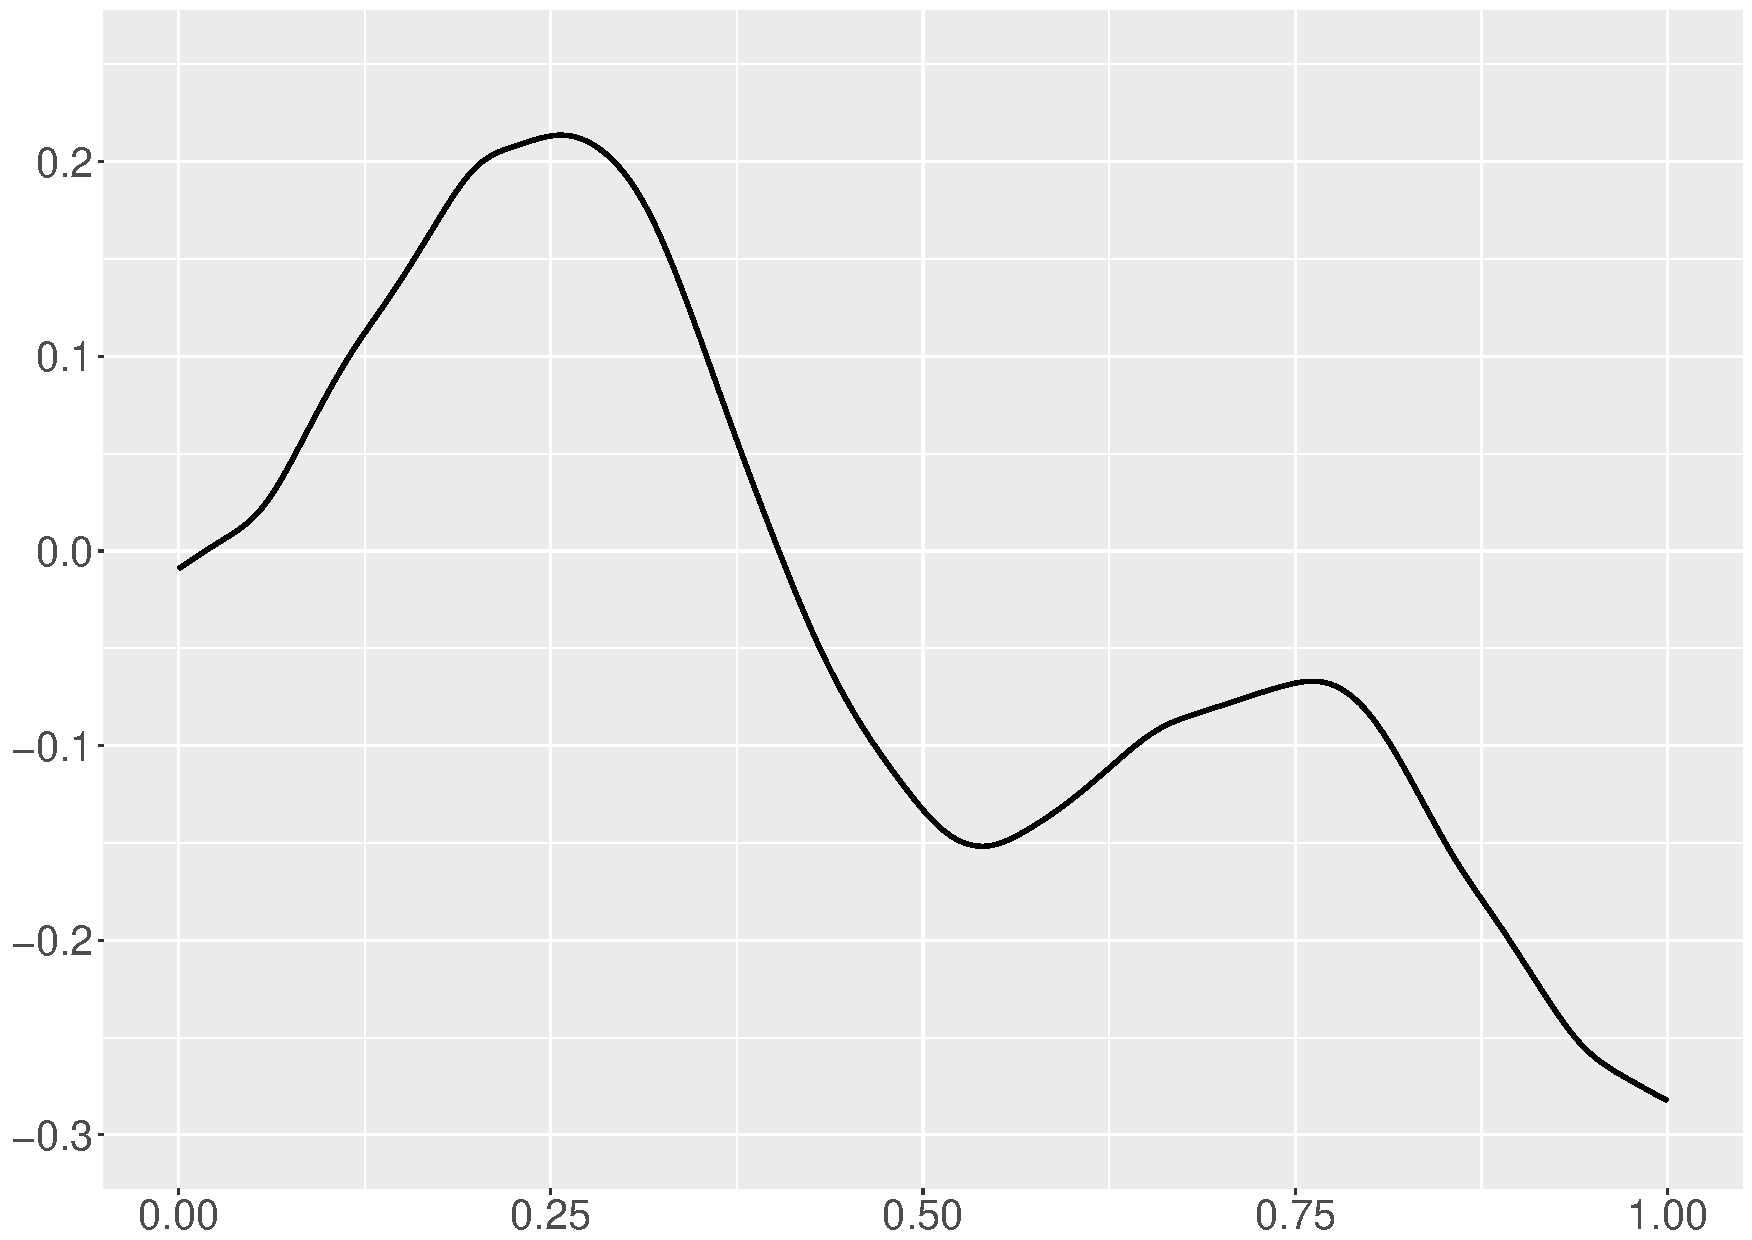
\includegraphics[width=5cm,height=3.5cm]{../Chapters/02TractorSplineTheory/plot/ggplot/ggHeaviSinePSpline}
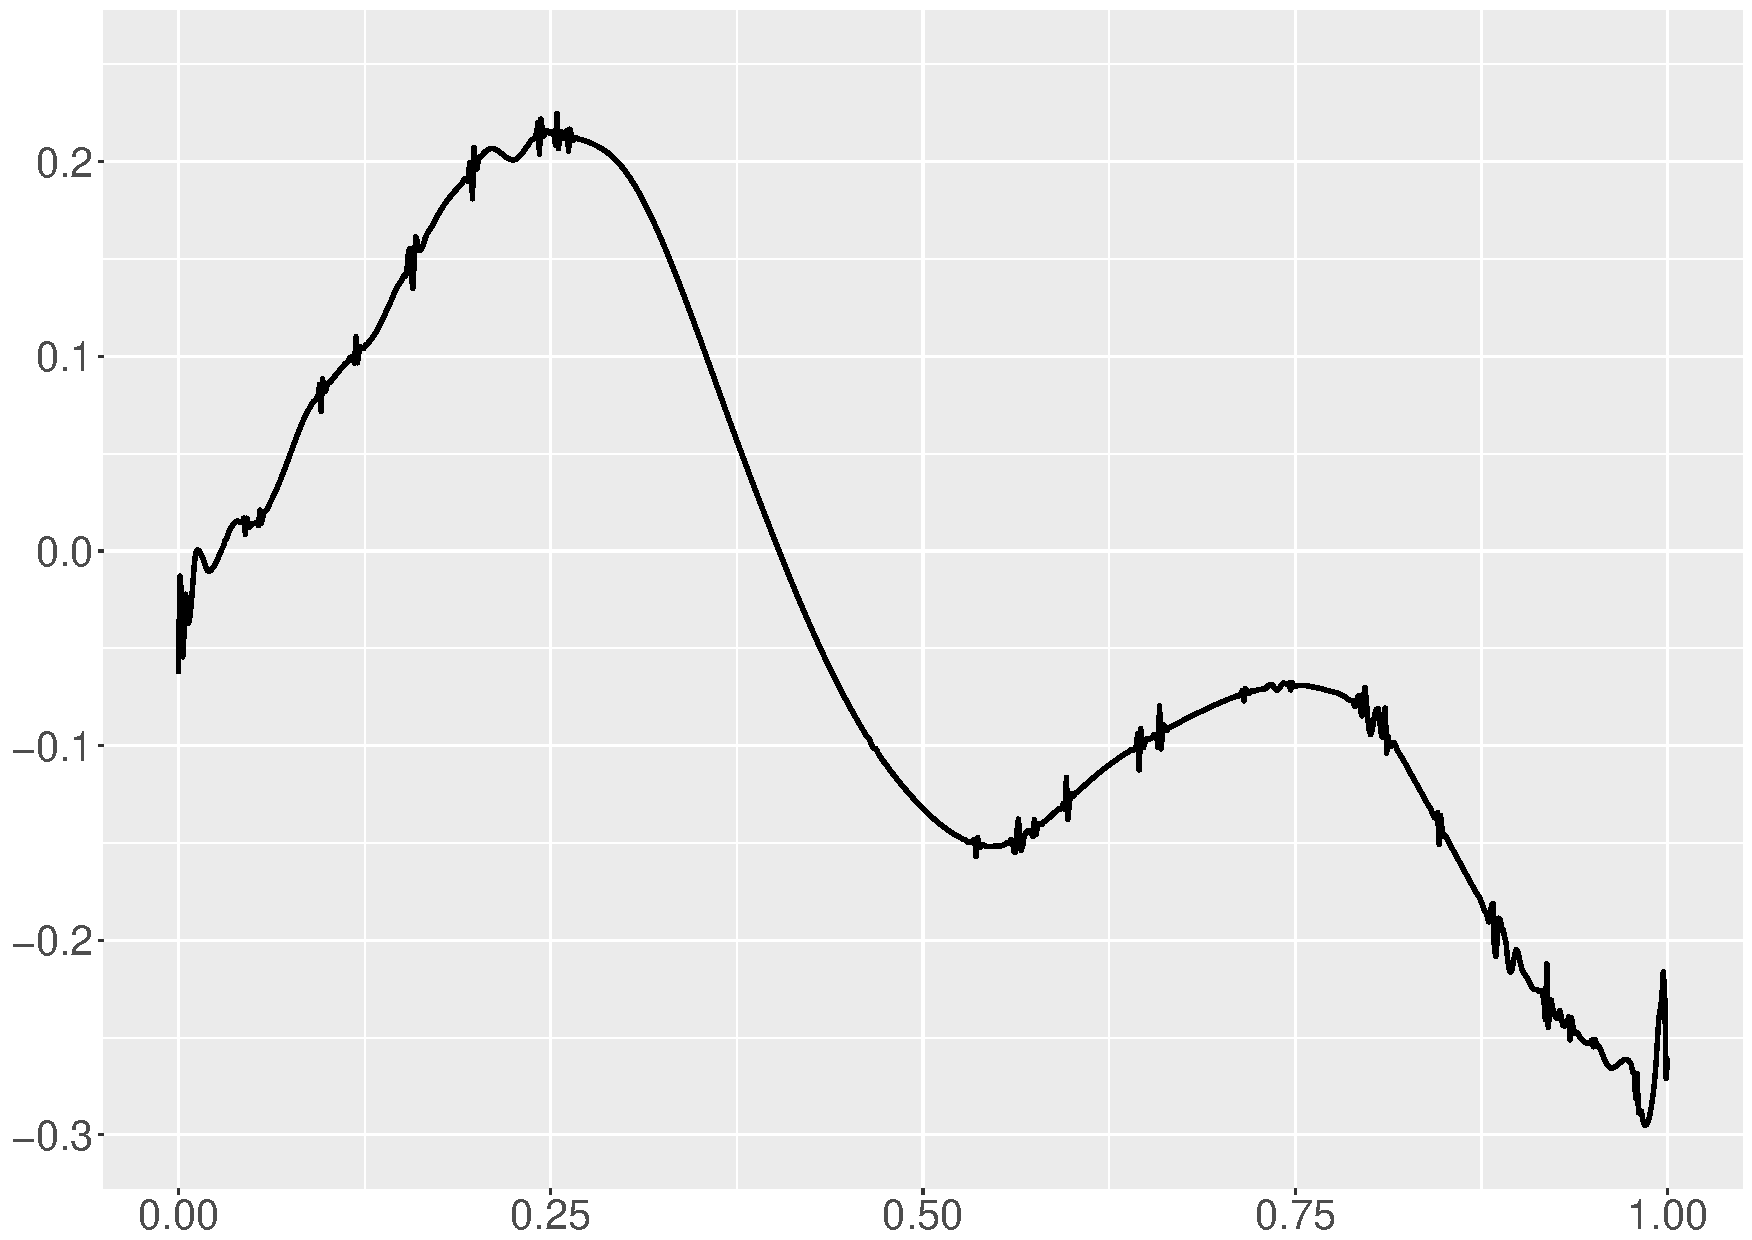
\includegraphics[width=5cm,height=3.5cm]{../Chapters/02TractorSplineTheory/plot/ggplot/ggHeaviSineSure}
\end{figure}
\end{frame}
%--------------------------------------------------------------------------------------
%--------------------------------------------------------------------------------------
\begin{frame}
\begin{figure}
\centering
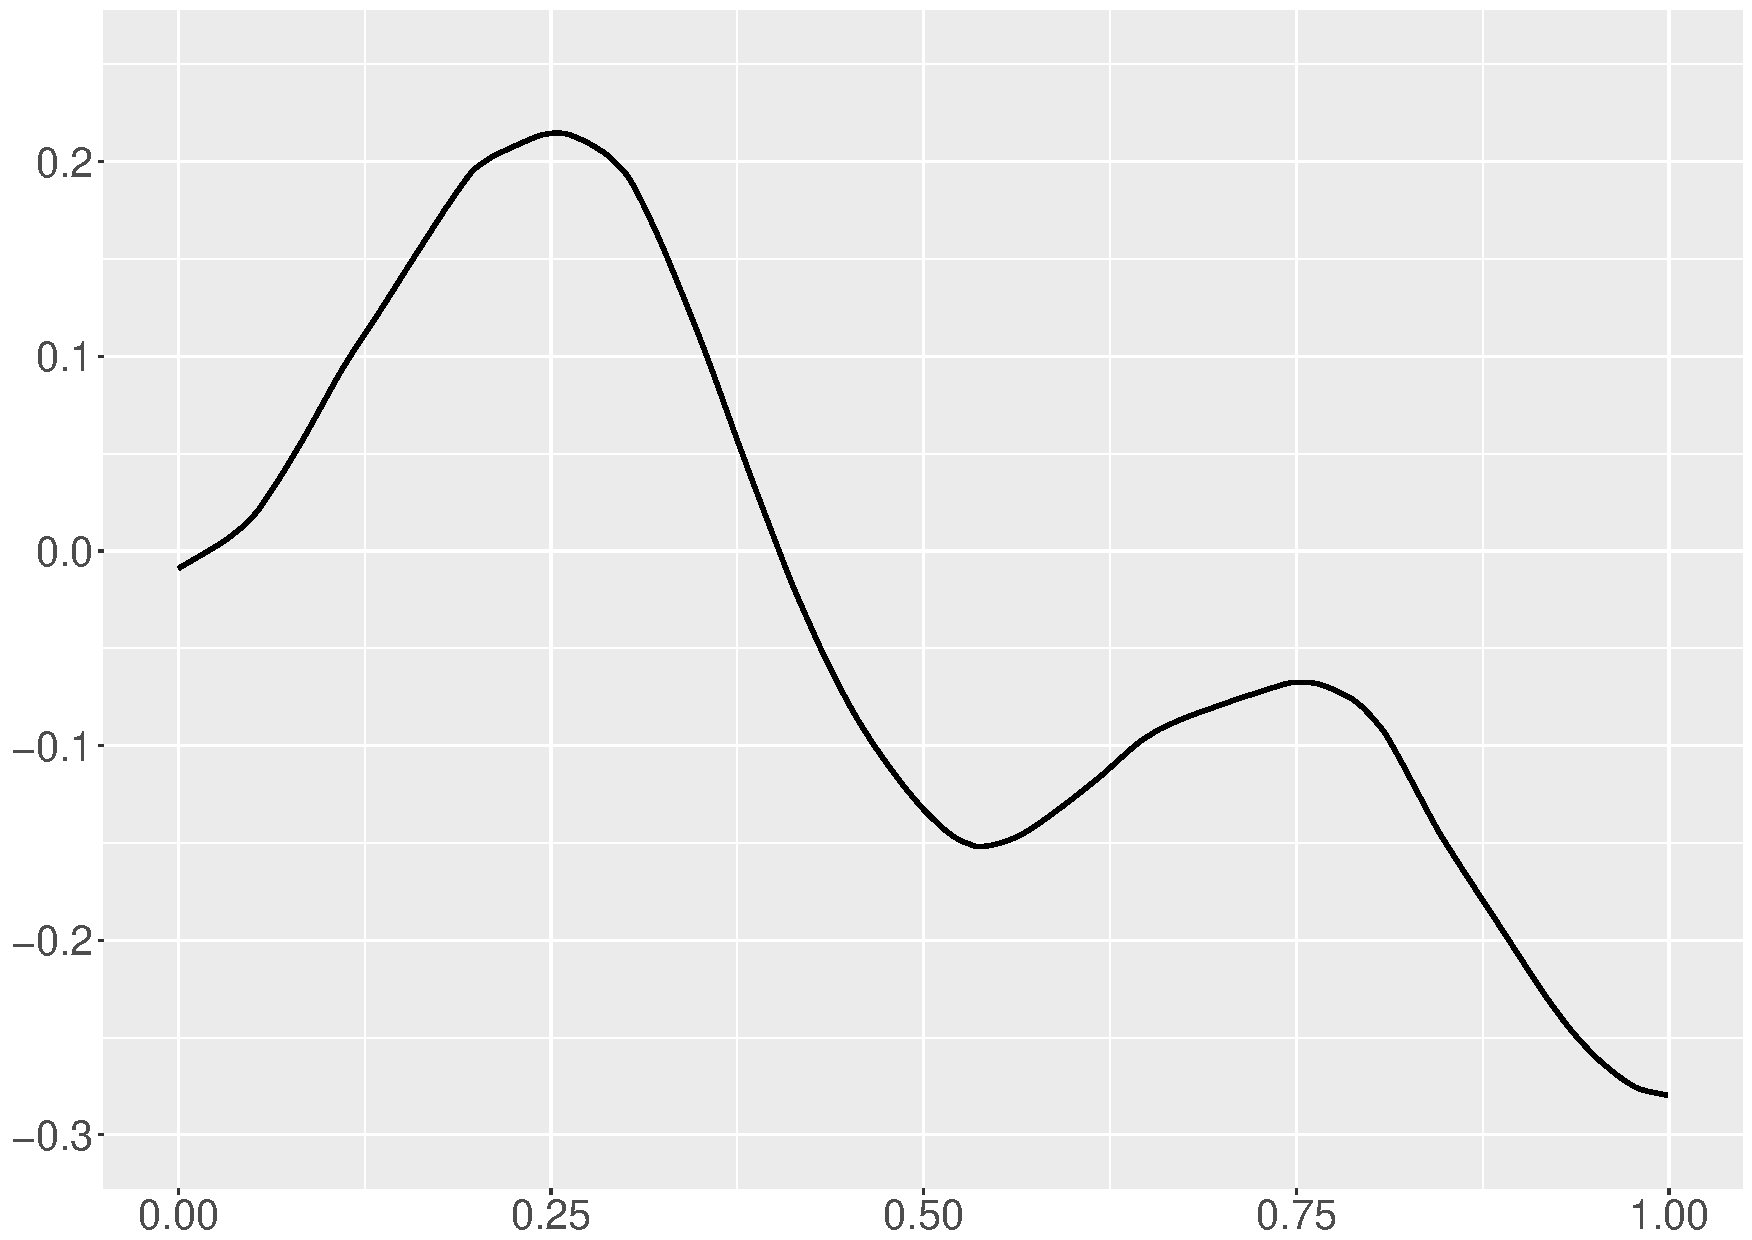
\includegraphics[width=5cm,height=3.5cm]{../Chapters/02TractorSplineTheory/plot/ggplot/ggHeaviSineGamma}
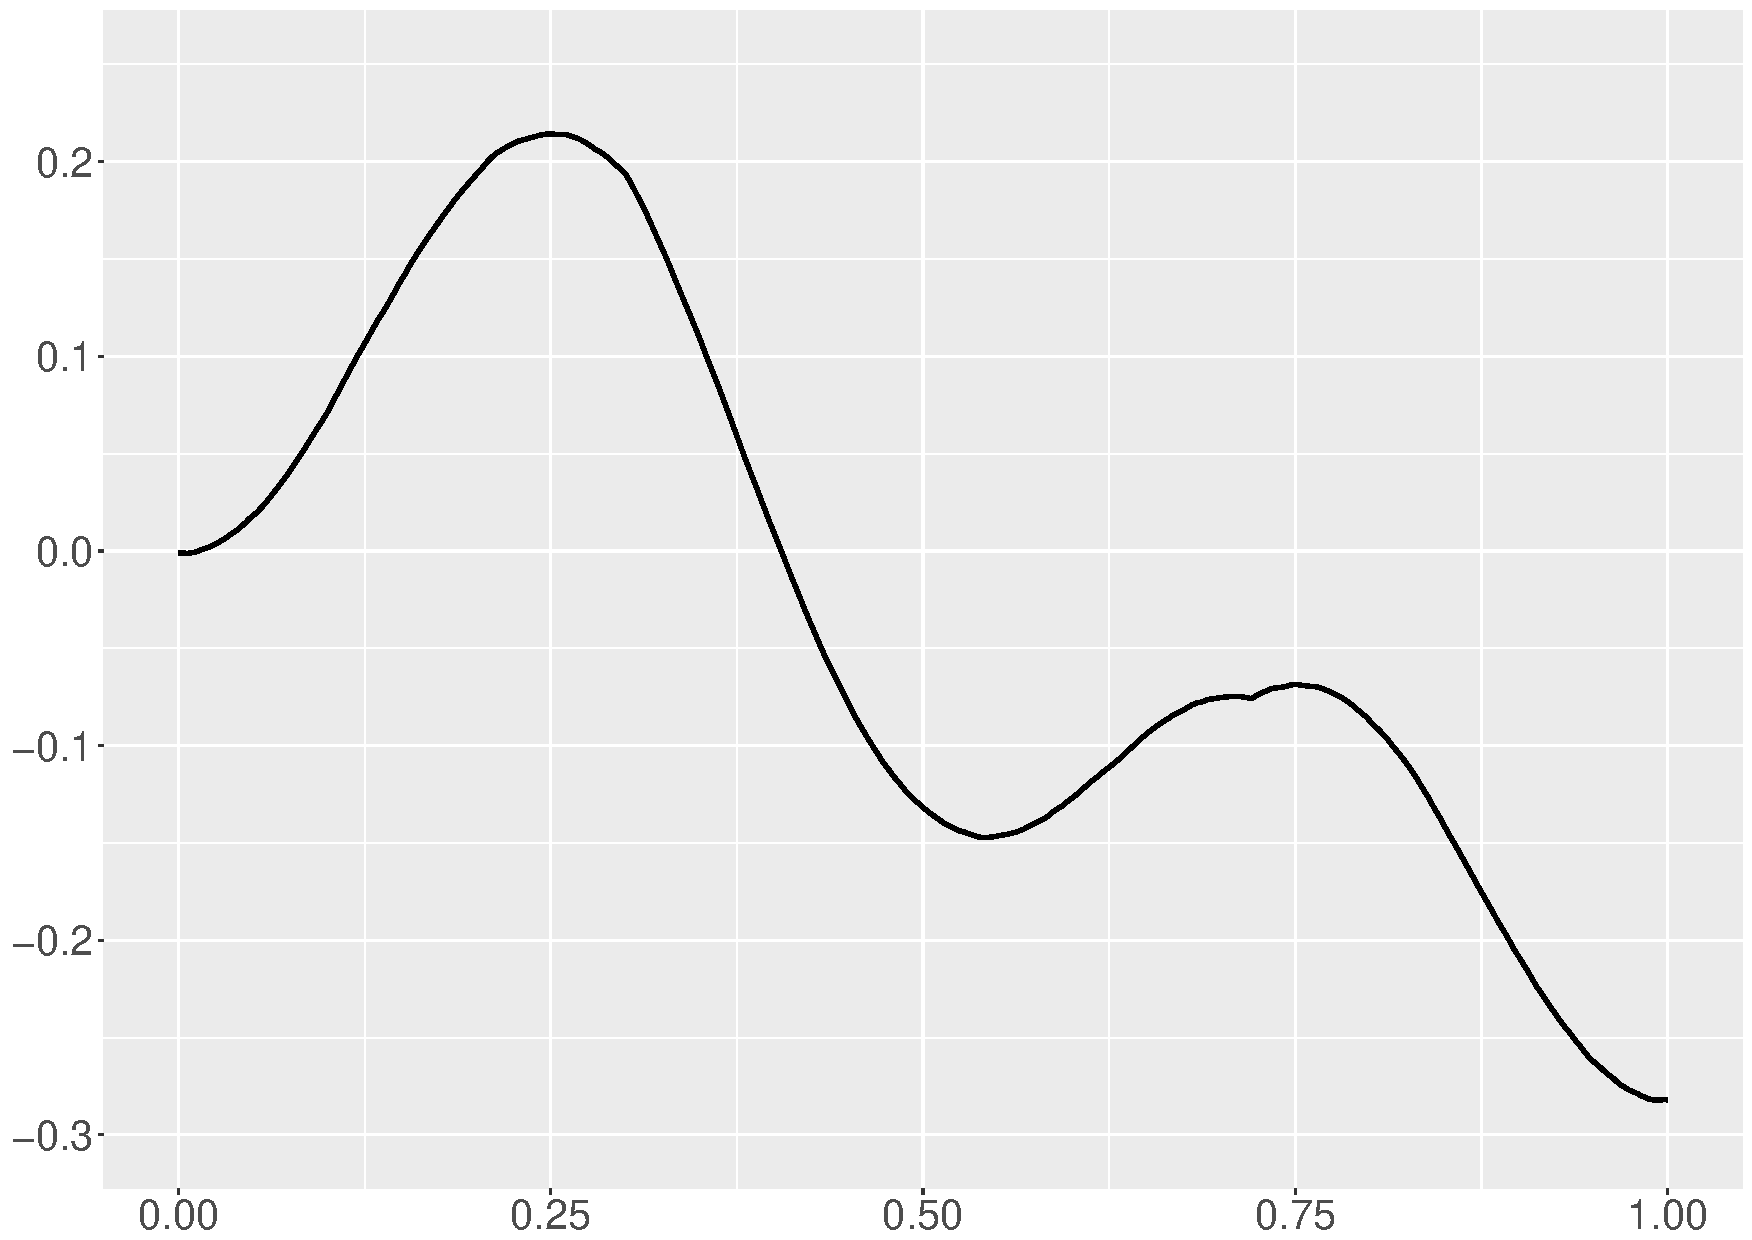
\includegraphics[width=5cm,height=3.5cm]{../Chapters/02TractorSplineTheory/plot/ggplot/ggHeaviSineTractorAPT}\\
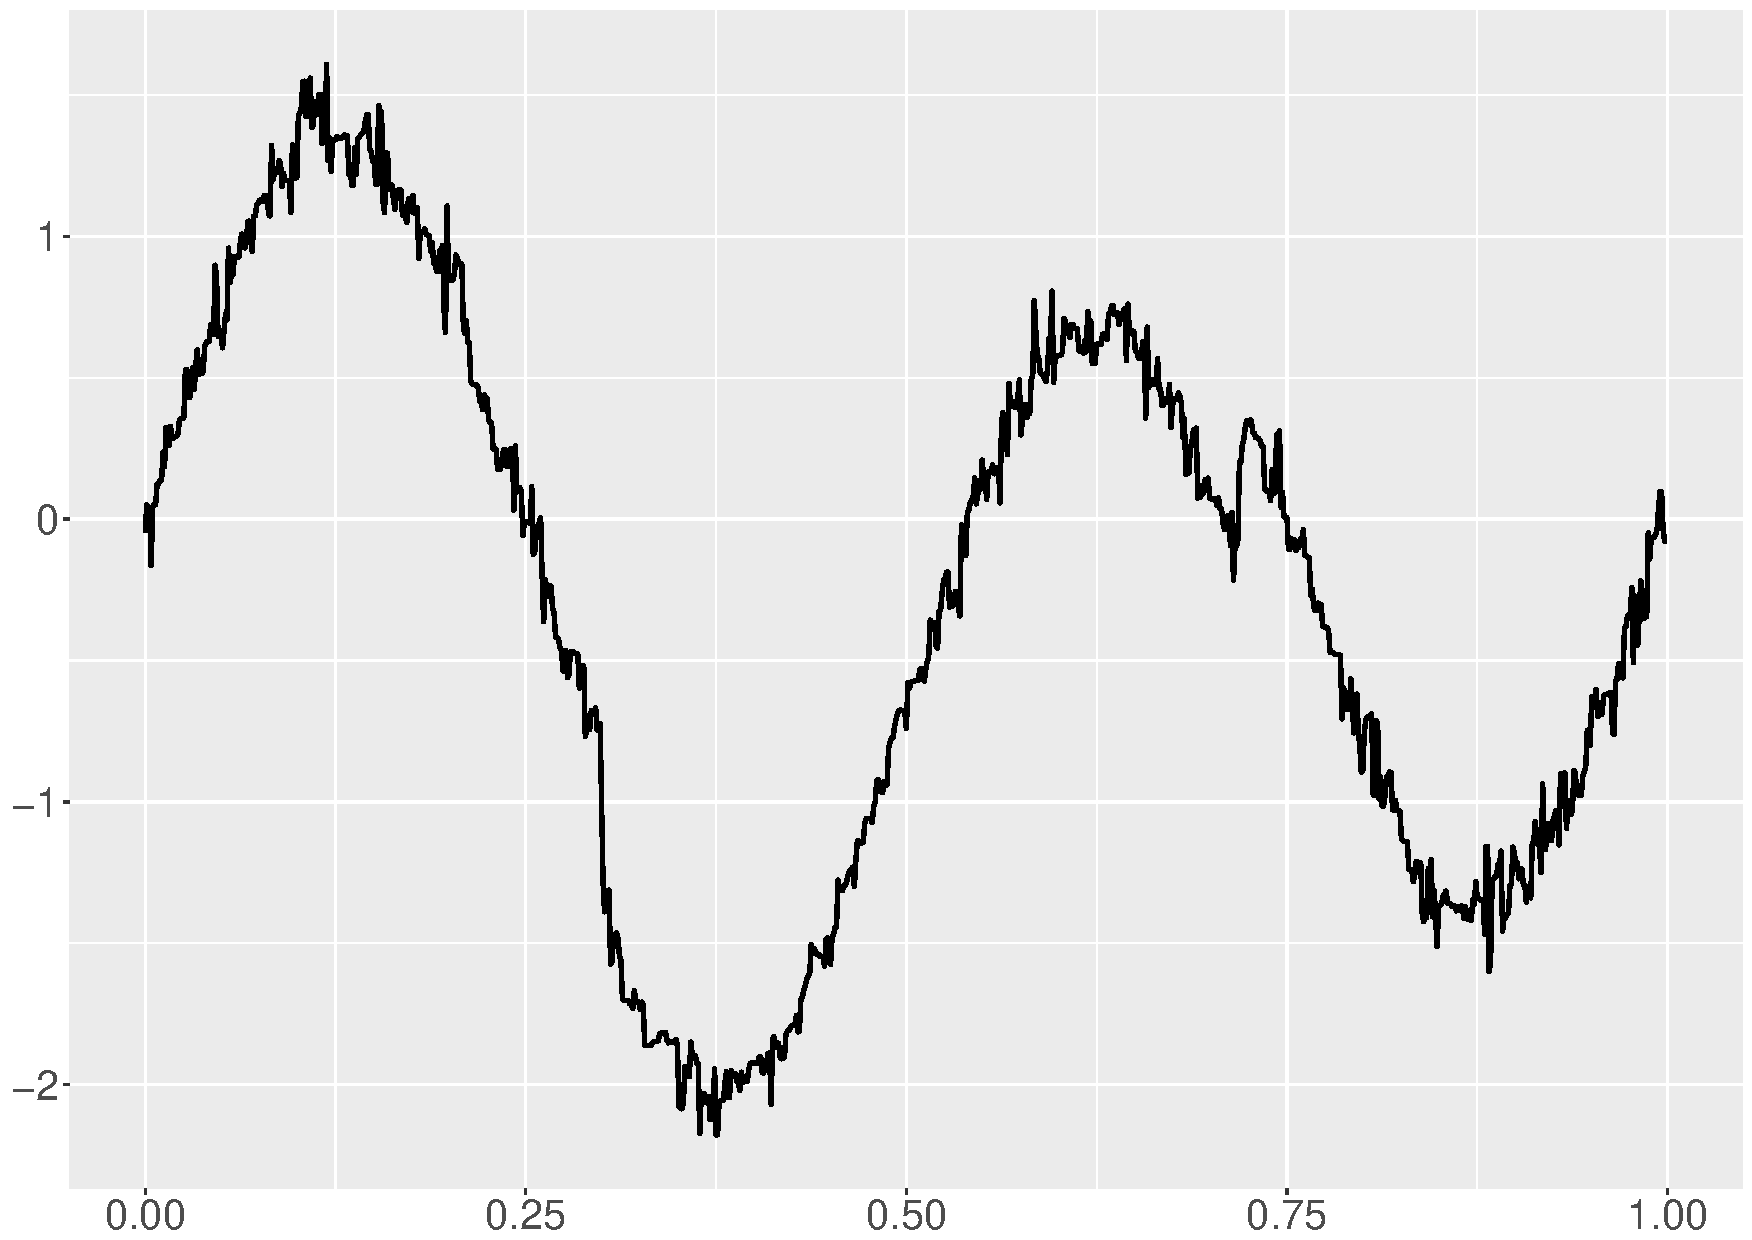
\includegraphics[width=5cm,height=3.5cm]{../Chapters/02TractorSplineTheory/plot/ggplot/ggHeaviSineTractorVelocity}
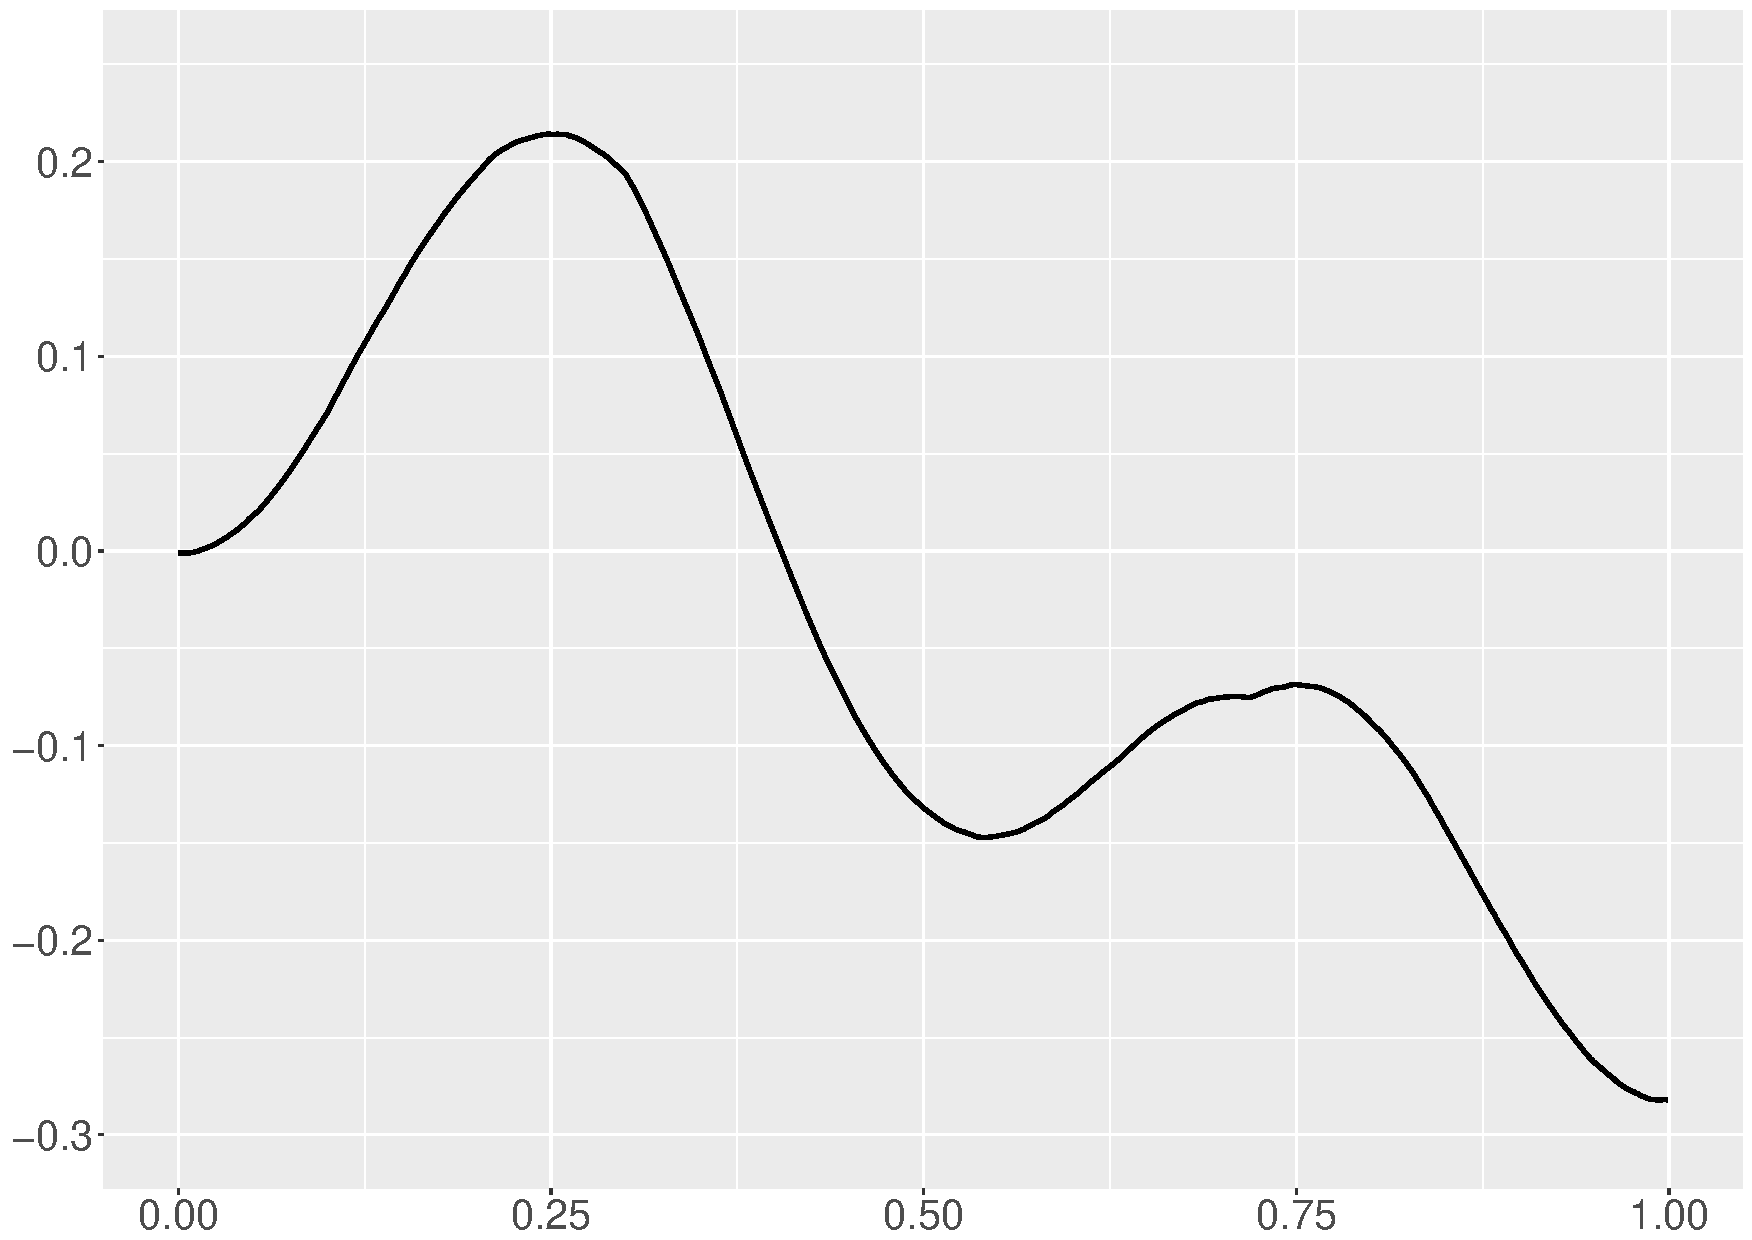
\includegraphics[width=5cm,height=3.5cm]{../Chapters/02TractorSplineTheory/plot/ggplot/ggHeaviSineTractor}
\end{figure}
\end{frame}
%--------------------------------------------------------------------------------------
%--------------------------------------------------------------------------------------

\begin{frame}

\begin{figure}
\centering
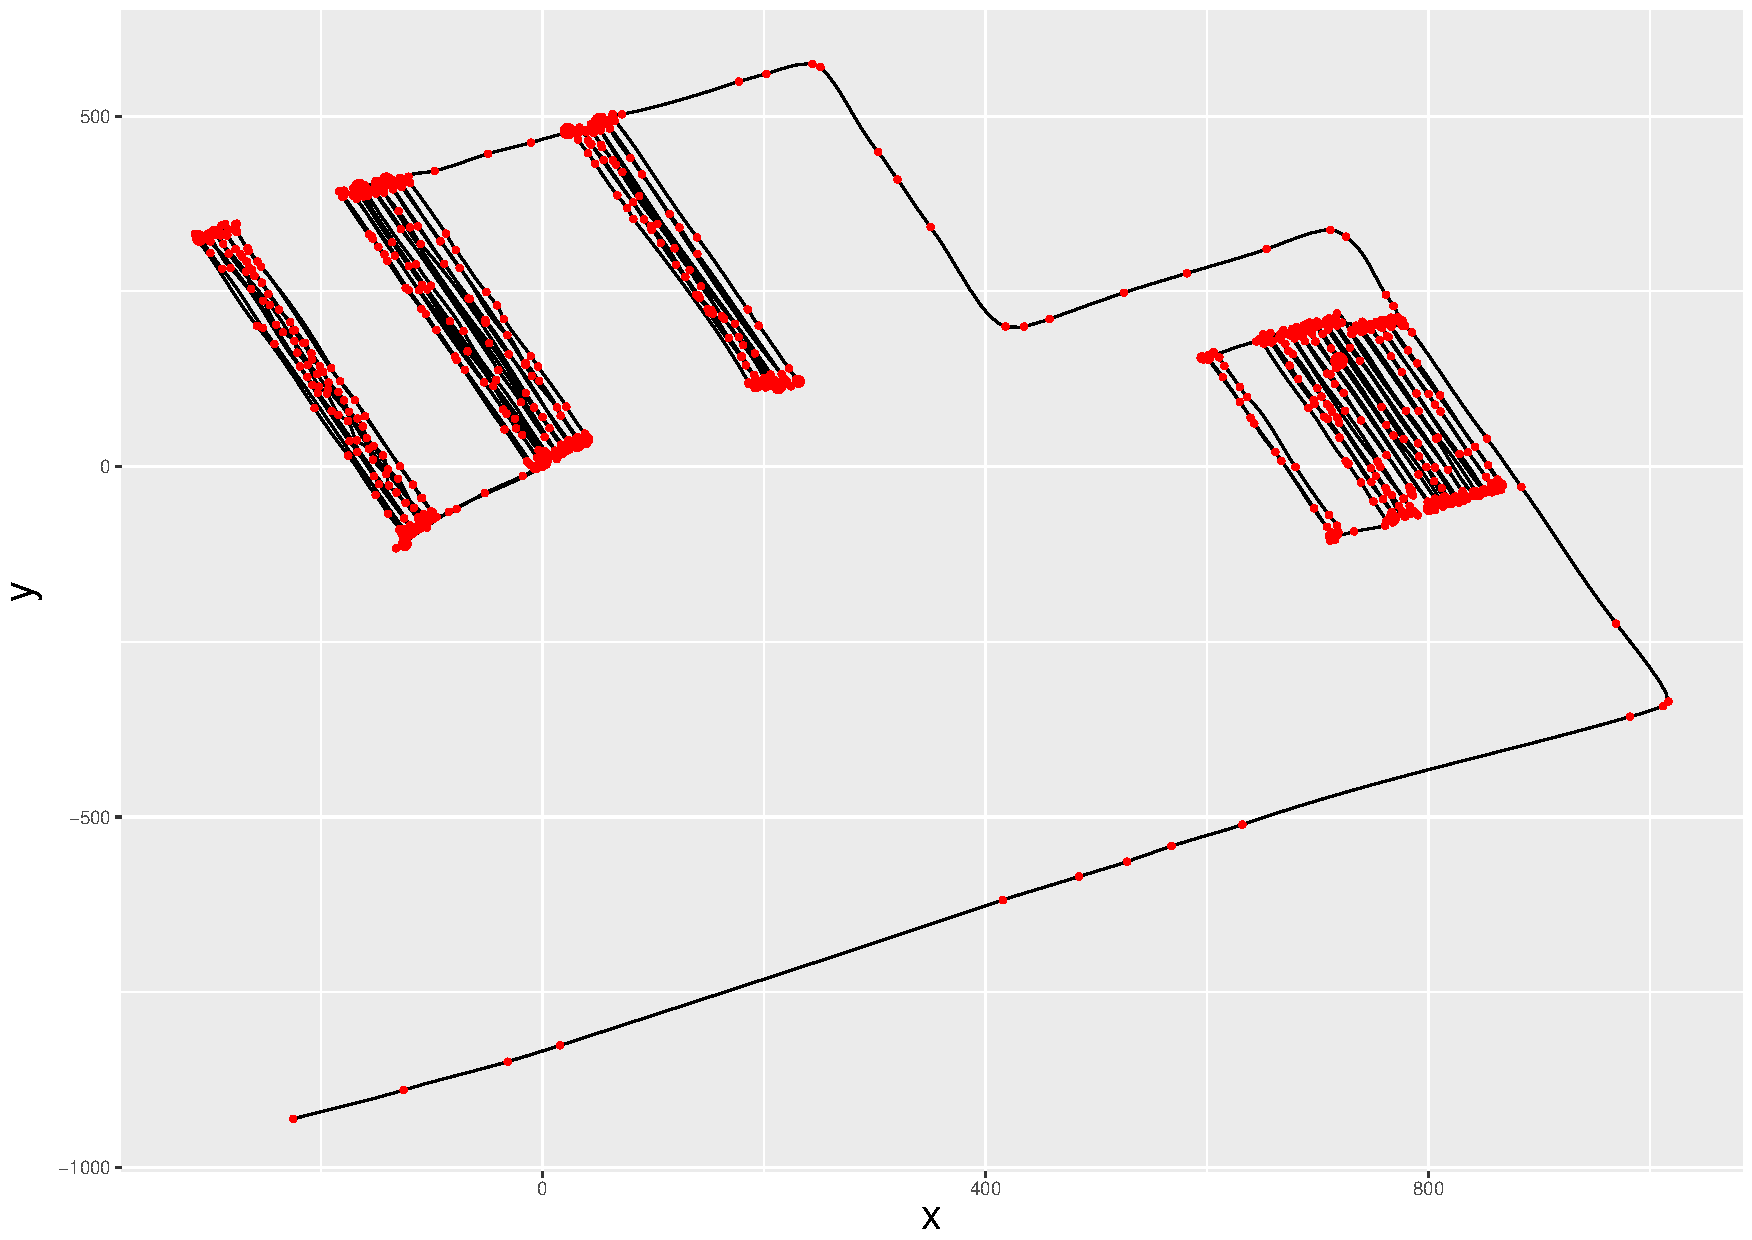
\includegraphics[width=0.9\linewidth]{../Chapters/02TractorSplineTheory/plot/ggplot/ggRealdataCompleteXY.pdf}
\caption{2-dimensional reconstruction. Larger dots indicate bigger values of penalty function $\lambda(t)$.}
\end{figure}

\end{frame}

%--------------------------------------------------------------------------------------
%--------------------------------------------------------------------------------------

\section{Adaptive Sequential MCMC}

\begin{frame}
\frametitle{On-line Estimation and Adaptive Sequential MCMC}


The forward map for the states is based on an Ornstein-Uhlenbeck process,
\begin{equation}\label{OUprocess}
\begin{cases}
\text{d}u_t = -\gamma u_t \text{d}t+ \lambda \text{d}W_t',\\
\text{d}x_t = u_t \text{d}t+\xi \text{d}W_t,
\end{cases}
\end{equation}
so that $\gamma^{-1}$ is roughly the time scale over which the velocity remains informative in the absence of subsequent observations. In our application, $\gamma^{-1}\approx 60\text{s}$.

The set of parameters to be estimated is $\theta=\{\gamma,\xi^2,\lambda^2,\sigma^2,\tau^2 \}$. The filtering for states is
\begin{equation}\label{filterX}
p(X_t\mid Y_{1:t}) = \int p(X_t\mid Y_{1:t} ,\theta)p(\theta \mid Y_{1:t})\text{d}\theta
\end{equation}
and $p(\theta\mid Y_{1:t}) \propto p(Y_{1:t}\mid \theta)p(\theta)$.

\end{frame}

%--------------------------------------------------------------------------------------

\begin{frame}
\frametitle{Learning Phase}

In the learning phase, a cheap Gaussian surrogate $\hat{p}(\theta)$ is obtained that will be used for a \textit{delayed-acceptance Metropolis-Hastings} sampler in the estimation phase. 

Specifically, a self-tuning random walk Metropolis-Hastings algorithm, in which the parameters are updated one at a time, is used to obtain the mean and covariance structure of $\hat{p}(\theta)$  

\end{frame}

\begin{frame}
\frametitle{Estimation Phase}

We use a Monte Carlo estimate of the target in \eqref{filterX}:
\begin{equation}
p(X_t\mid Y_{1:t}) \dot{=} \frac{1}{N}\sum_{i=1}^{N}p(X_t\mid Y_{1:t},\theta^{(i)}). 
\end{equation}

To maintain sampling speed, we introduce a \textit{Sliding Window MCMC} algorithm that retains only the last $L$ observations. This is also advantageous in our application as the parameters are often slowly varying in time. To maintain sampling efficiency, if the acceptance ratio $\alpha$ drops below a predefined threshold, the mean of $\hat{p}(\theta)$ is updated (the covariance is kept the same). 

\end{frame}






\begin{frame}
\frametitle{Application}
A tractor moving on an orchard is mounted with a GPS-enabled unit, which records
and transmits data to a remote server. The data is an irregularly spaced time series of longitude, latitude, speed and bearing. In online mode, the sliding window algorithm is able to infer the tractor's position within seconds with an uncertainty of $\approx 0.5\text{m}$. A window $L$ of 100 is chosen to maintain a balance between sampling speed and acceptable estimation errors. 
\end{frame}

%--------------------------------------------------------------------------------------
%--------------------------------------------------------------------------------------


\begin{frame}
For the priors of all the parameters in an OU-process, the reciprocal of $\gamma$ is typical velocity falling in the reasonable range of 0.1 to 100 $m/s$. $\xi$ is the error occurs in transition process, $\sigma$ and $\tau$ are errors in the forward map for position and velocity respectively. 
\begin{align*}
\gamma   &\sim IG(10,0.5),\\
\xi^2        &\sim IG(5,2.5),\\
\sigma^2 &\sim IG(5,2.5),
\end{align*}
where $IG(\alpha,\beta)$ represents the \textit{Inverse Gamma} distribution with two parameters $\alpha$ and $\beta$. 
%\begin{figure}[h]
%\centering
%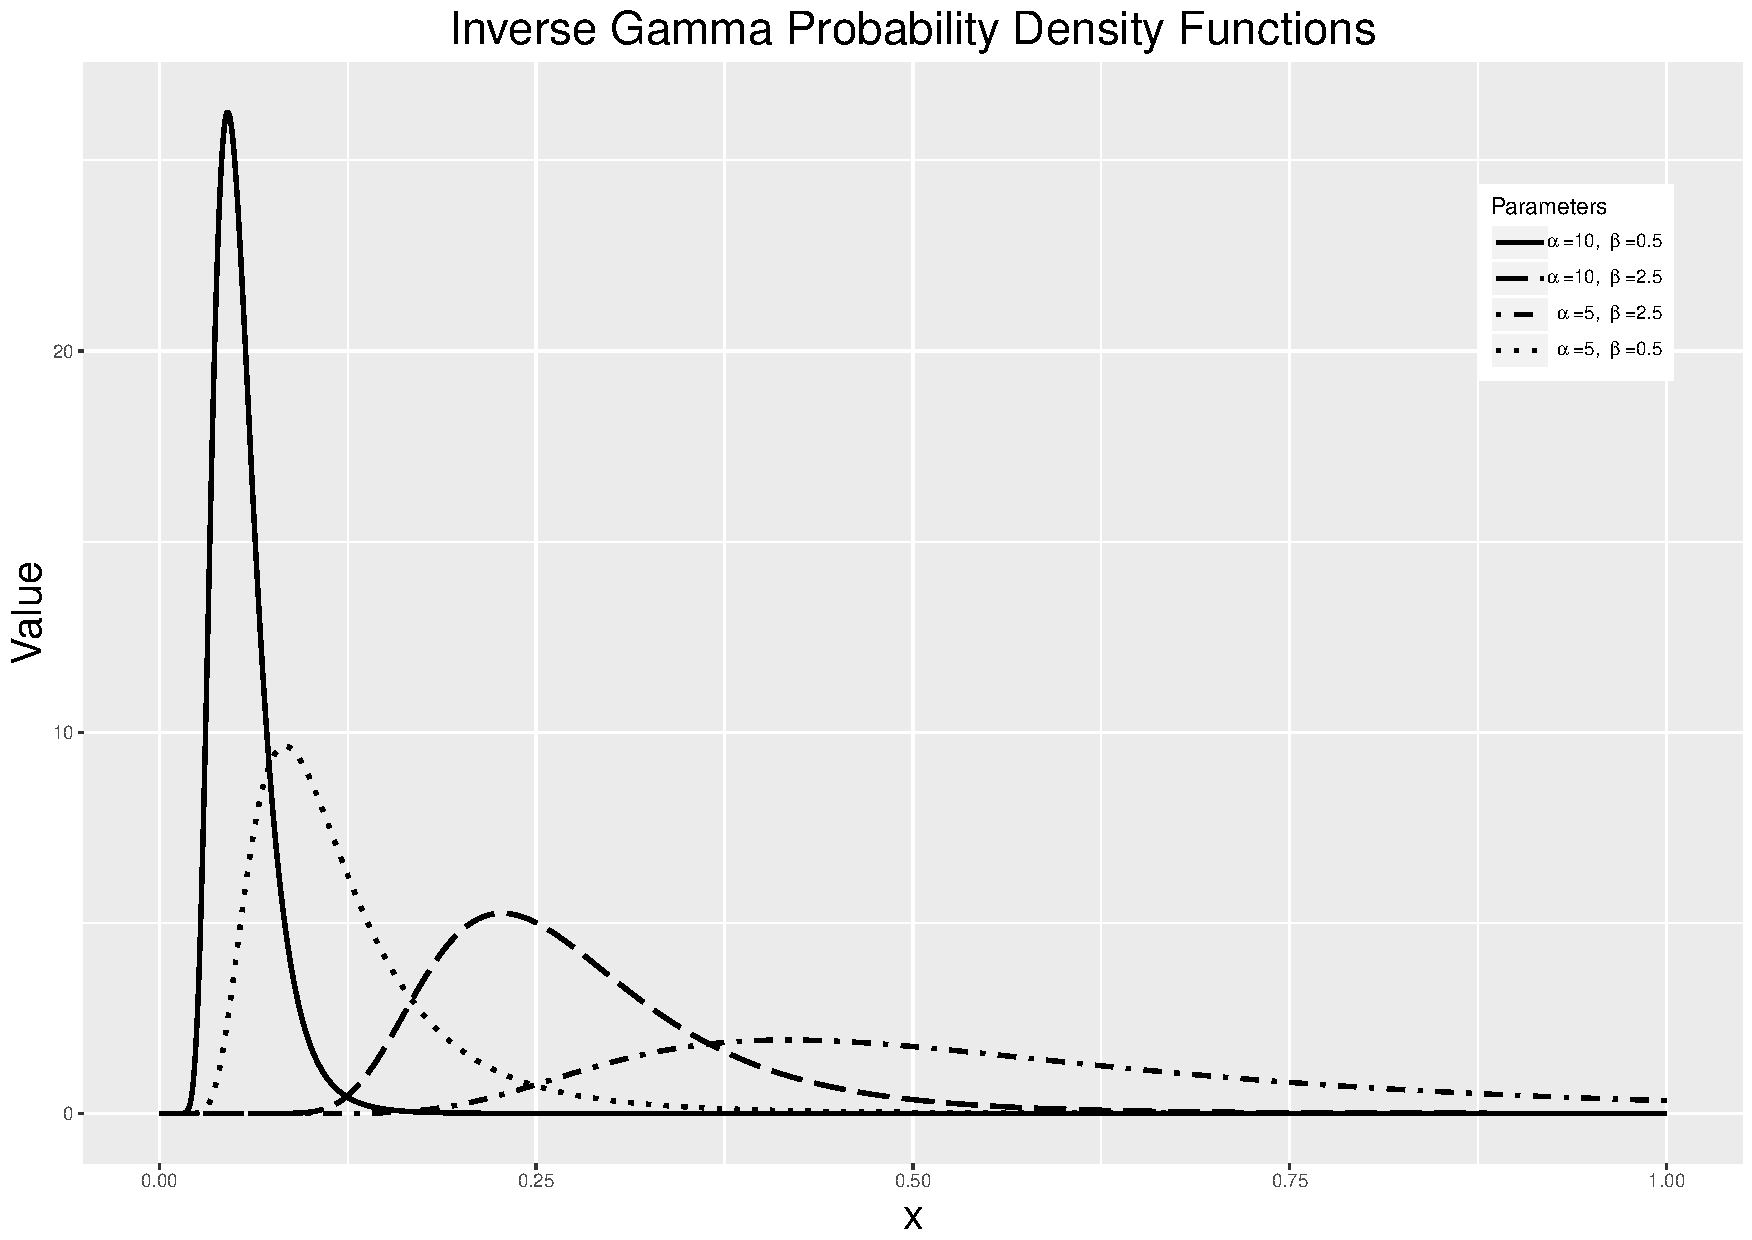
\includegraphics[width=0.45\textwidth]{Chapters/05MCMCOU/plots/ggIGPDF.pdf}
%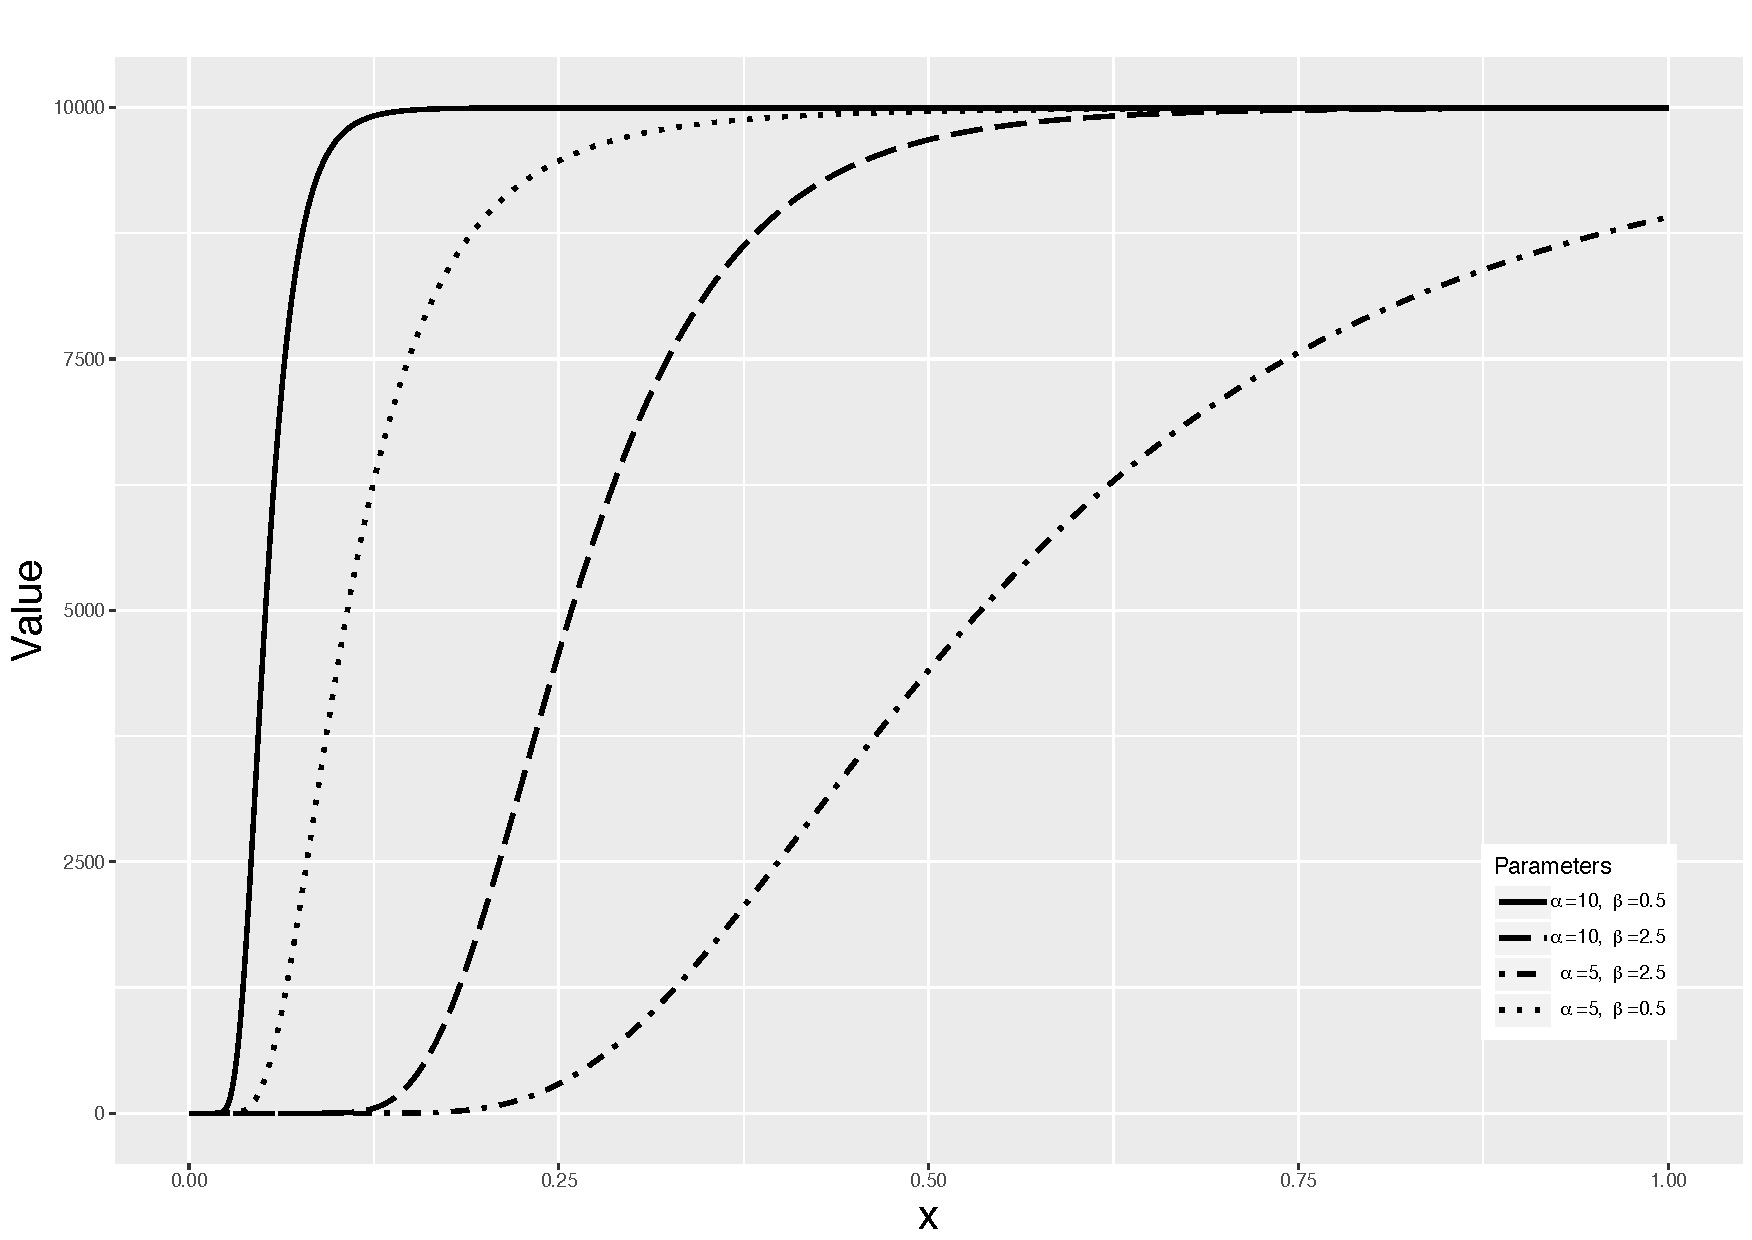
\includegraphics[width=0.45\textwidth]{Chapters/05MCMCOU/plots/ggIGCDF.pdf}
%\caption{Probability density function and cumulative distribution function of \textit{Inverse Gamma} with two parameters $\alpha$ and $\beta$. }
%\label{IGPDFCDF}
%\end{figure}
\end{frame}

%--------------------------------------------------------------------------------------
%--------------------------------------------------------------------------------------

\begin{frame}
\begin{figure}[h]
\centering
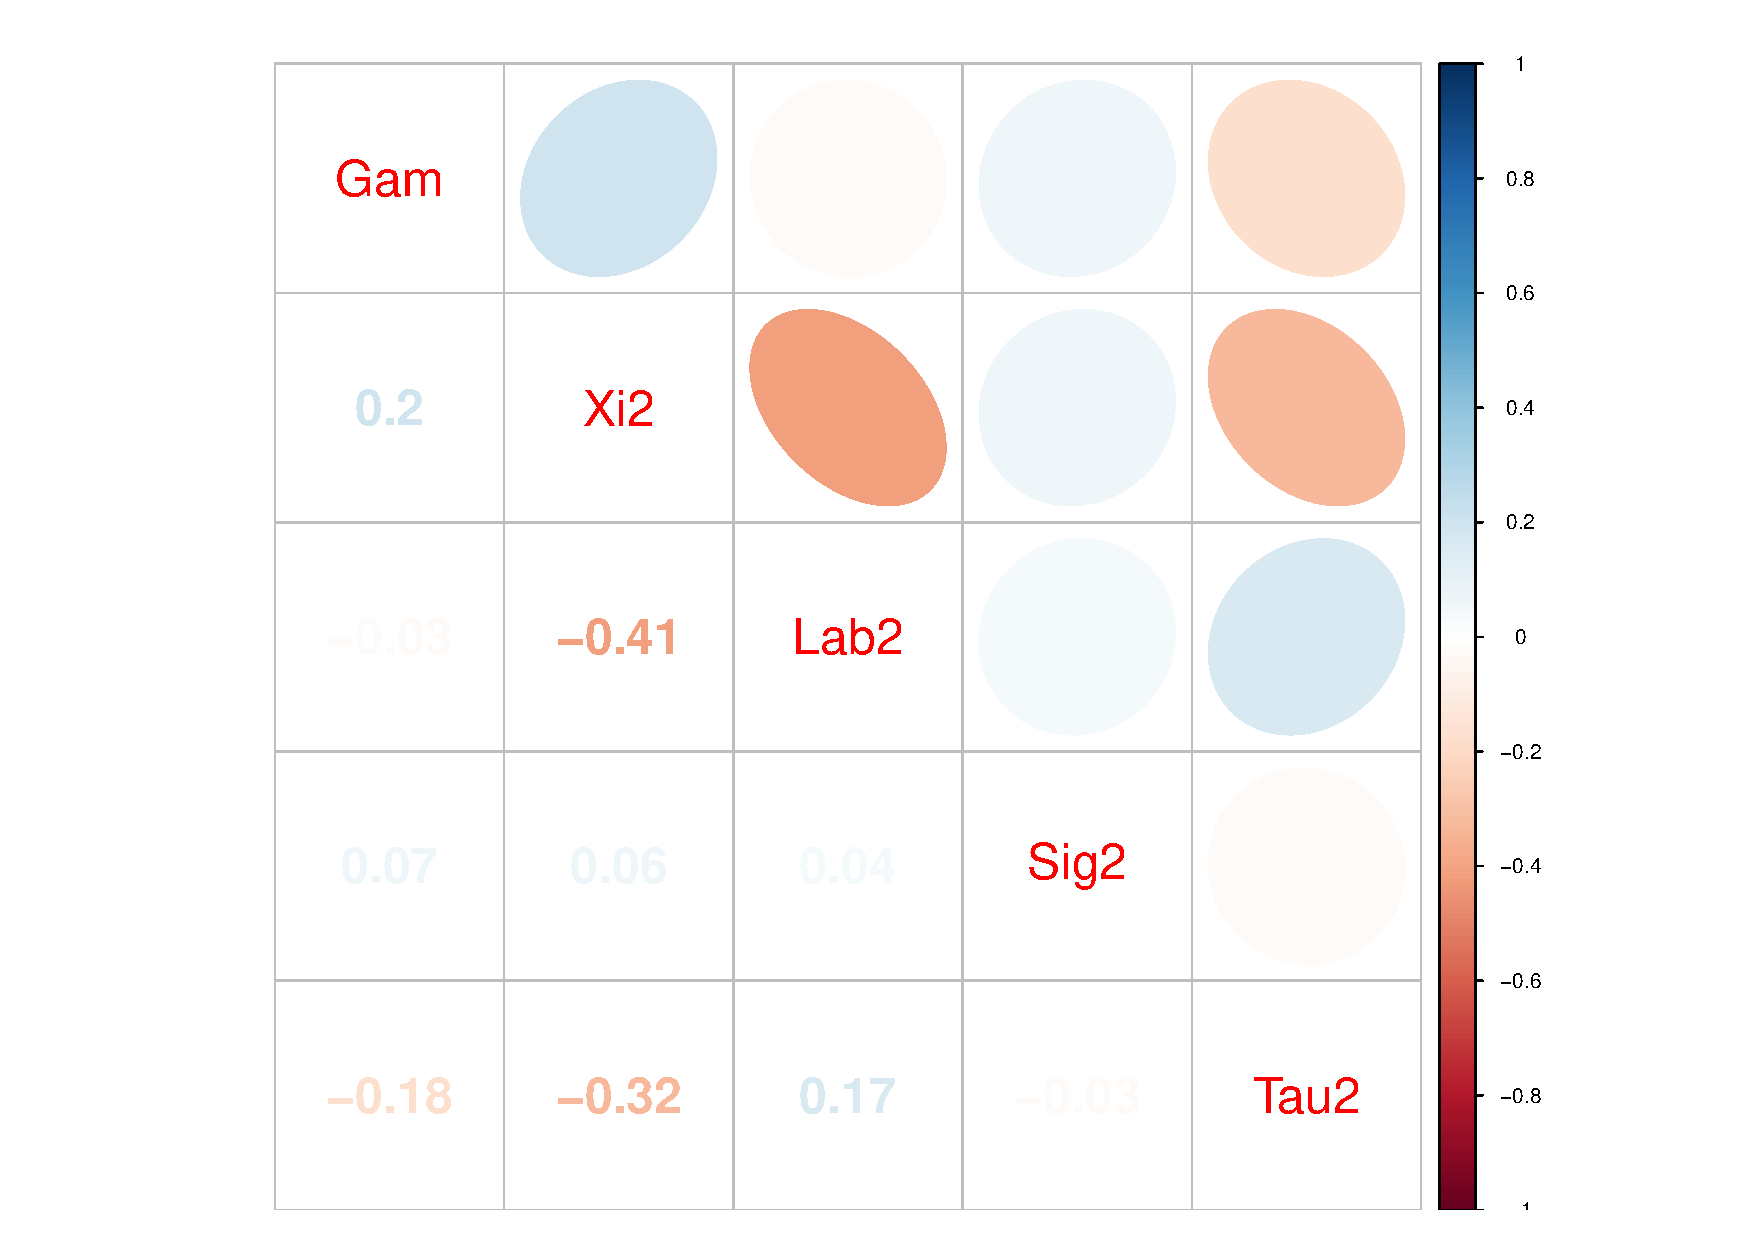
\includegraphics[width=0.8\textwidth]{../Chapters/05MCMCOU/plots/realdatalearningcorMatrix.pdf}
\caption{Visualization of the parameters correlation matrix, which is found in learning phase. }\label{realdatacorMatrix}
\end{figure}

\end{frame}

%--------------------------------------------------------------------------------------
%--------------------------------------------------------------------------------------


\begin{frame}


\begin{figure}[h]
	\centering
	\begin{tikzpicture}
	\node[anchor=south west,inner sep=0] (image) at (0,0) {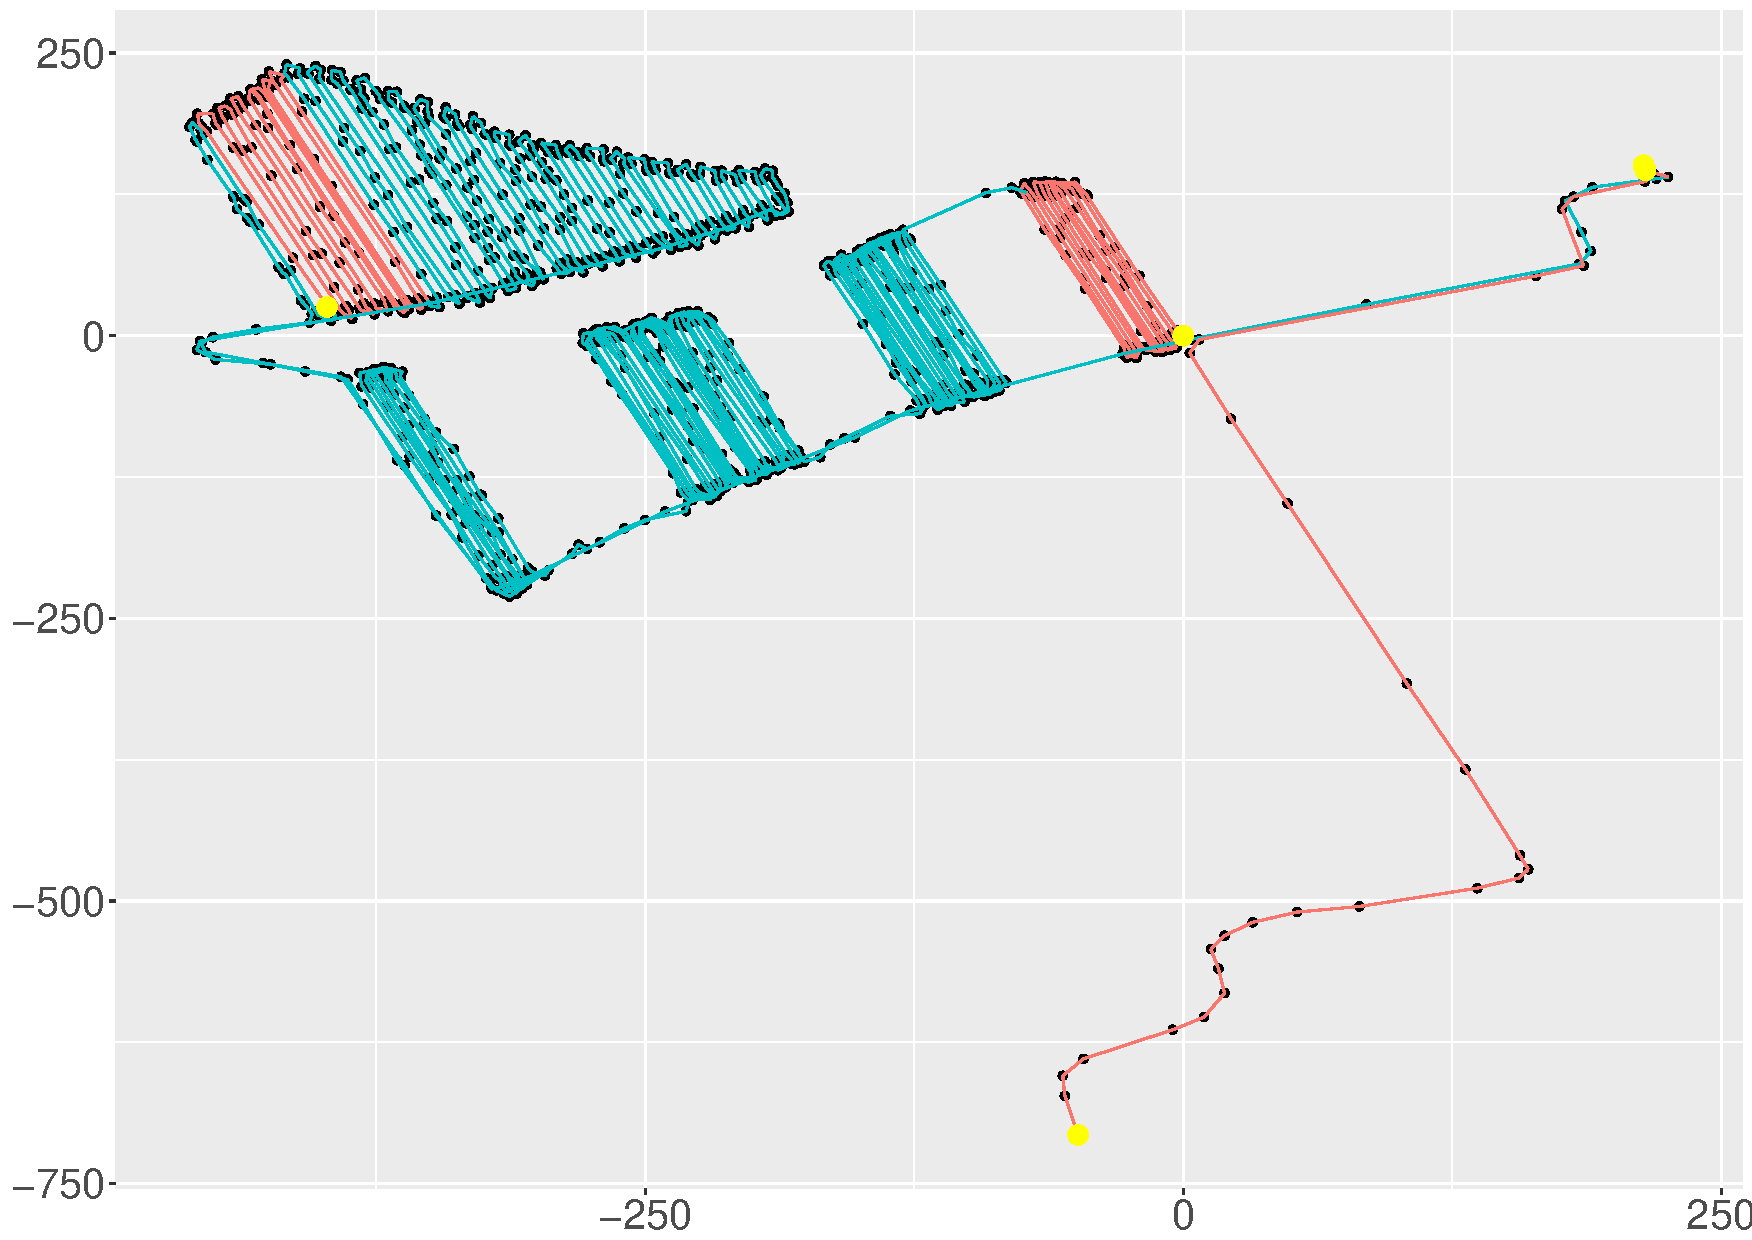
\includegraphics[width=0.9\textwidth]{../Chapters/05MCMCOU/plots/realdatabatchPositionwhole2.pdf}};
	\begin{scope}[
	x={(image.south east)},
	y={(image.north west)}
	]
	\node [black, font=\bfseries] at (0.5,0) {Easting};
	\node [black, font=\bfseries,rotate=90] at (0,0.5) {Northing};
	\node [black, font=\bfseries] at (0.68,0.68) {1};
	\node [black, font=\bfseries] at (0.15,0.75) {2};
	\node [black, font=\bfseries] at (0.94,0.83) {3};
	\node [black, font=\bfseries] at (0.64,0.08) {4};
	\end{scope}
	\end{tikzpicture}
	%\caption{Two learning phases are colored by red and two sequential estimation phases are colored by green. The algorithm is not able to estimate the data from 1121 till the end because of the lack of observations. Point 1 is the first point of the data stream. Points 2 and 3 are the switching points. Point 4 is the last point of the data stream. }\label{MCMCwholeestimation}
\end{figure}


\end{frame}

%--------------------------------------------------------------------------------------
%--------------------------------------------------------------------------------------




\begin{frame}

Further videos at:

\href{https://www.youtube.com/watch?v=lQOSt8HrYRU&t=61s}{V-spline reconstruction} 

\href{https://www.youtube.com/watch?v=CF6Sut3G6eI&t=67s}{Adaptive MCMC} 

\end{frame}


%--------------------------------------------------------------------------------------
%--------------------------------------------------------------------------------------


\begin{frame}
\frametitle{Amendments}
\begin{itemize}
	\item Chapter one: introduction for GPS data.
	\item Chapter two: larger labels in figures.
	\item Chapter three: the conjecture has been resolve.
	\item Chapter four: fixed typographical errors.
	\item Chapter five: explicit explanation, better figures.
	\item Others: references are properly cited.
\end{itemize}


\end{frame}


%--------------------------------------------------------------------------------------
%--------------------------------------------------------------------------------------

\begin{frame}
\frametitle{Acknowledgment}
\begin{itemize}
\item Ministry of Business, Innovation \& Employment\\
 \hskip 0.5cm -- Grant UOOX 1208\\
\item TracMap\\
\item Dr Matthew Parry\\
\item Professor David Bryant \\
\item All ex000aminers 
\end{itemize}
\end{frame}

%--------------------------------------------------------------------------------------
%--------------------------------------------------------------------------------------

\begin{frame}
\begin{figure}
\centering

\includegraphics[]{plots/mbie}\\

\includegraphics[]{plots/tracmap-agriculture}
\centering
\end{figure}
\end{frame}

%--------------------------------------------------------------------------------------


%
%\section{References}
%\begin{frame}
%\frametitle{6 References}
%\footnotesize{
%\begin{thebibliography}{99} % Beamer does not support BibTeX so references must be inserted manually as below
%\bibitem[2001]{b1} T. Hastie, R. Tibshirani, J. Friedman, and J. Franklin  (2001)
%\newblock The Elements of Statistical Learning: data mining, inference and prediction.
%%\newblock \emph{Biometrika} 62(1):79-88.
%
%\bibitem[1978]{b2} P. J. Green. (1994)
%\newblock Nonparametric regression and generalized linear models : a roughness penalty approach
%%\newblock \emph{Journal of the Royal Statistical Soceity} N, 40:1-42.
%
%\bibitem[1978]{p1} Y.J. Kim and C. Gu (2004)
%\newblock Smoothing spline gaussian regression: more scalable computation via efficient approximation
%\newblock \emph{ Journal of the Royal Statistical Society: Series B (Statistical Methodology)} vol. 66,
%no. 2, pp. 337-356
%
%\bibitem[Blight and Ott 1975]{b3} Blight, B.J.N. and Ott, L. (1975)
%\newblock A Bayesian Approach to Model Inadequacy for Polynomial Regression.
%\newblock \emph{Biometrika} 62(1):79-88.
%
%\bibitem[2008]{b4} G.P.Nason. (2008)
%\newblock Wavelet Methods in Statistics with R.
%\end{thebibliography}
%}
%\end{frame}

%------------------------------------------------

%
%\begin{frame}
%\frametitle{Future Research Plans in Academic Career}
%\begin{itemize}
%\item Gradient boosting V-spline: to speed up computation
%
%\item MCMC algorithms, such as adaptive MCMC, grid-based MCMC and parallel MCMC algorithms, subsample MCMC. 
%
%\item Computational biology: such as genotype imputation, epidemiological forecasting. 
%
%\item Statistical methodologies and their applications.  
%
%\end{itemize}
%
%\end{frame}


%\begin{frame}
%\Huge{\centerline{Thank you for your attention.}}
%\end{frame}

%----------------------------------------------------------------------------------------

\end{document} 